\section{Probabilistic Knowing How}\label{sec:prob}

\subsection{Linear Plans}\label{subsec:prob:linear}

Naturally, our first approach will be extending $\Khlogic$ with some
form of probabilistic behaviour.  For this, we first need to
understand how plans work in a probabilistic model.
%
Thus, given a plan $\plan\in\Act^*$, we want to consider
strategies that follow as faithfully as possible the plan
$\plan$. This is captured in the next definition.

\begin{definition}\label{def:plan:compat}
  A strategy $\strat$ is \emph{$\plan$-compatible} if for all
  $\rho\in\execf$ such that $\bar{\rho}\in\pref(\plan)$,
  %
  \begin{enumerate}
  \item%
    $\strat(\rho)(a,\mu)>0$ implies $\bar{\rho}a\in\pref(\plan)$, and
  \item%
    $\strat(\rho)(\complete)>0$ implies that either
    $\bar{\rho}=\plan$ or
    $\{\bar{\rho}a\mid{\last(\rho)\reach{a}\mu}\}\cap\pref(\plan) = \emptyset$. 
  \end{enumerate}
  %
  Let $\Comp(\plan)$ denote the set of all $\plan$-compatible
  strategies.
\end{definition}
%
The first item states that $\strat$ can chose an $a$-labeled
transition after the partial plan $\bar{\rho}$ if the continuation of
$\bar{\rho}a$ is also a partial plan.
%
The second item states that $\strat$ is allowed to terminate after the
partial plan $\bar{\rho}$ if either $\bar{\rho}$ is itself a valid
plan or $\bar{\rho}$ cannot be continued by the PLTS within the plan.

It is important to remark that, since $\plan$ is finite, for any
$\plan$-compatible strategy $\strat$ and state $s$,
$\Prob^\strat_s(\execw)=0$ (or equivalently,
$\Prob^\strat_s(\cexecf)=1$).  That is, any $\plan$-compatible
strategy leads to termination with probability $1$.
%
Also notice that in PFA, the strategy $\strat_\plan$ as defined in
\Cref{sec:preliminaries} is the only one $\plan$-compatible.  By
``only one'', we mean that any strategy defined so that it satisfy the
same conditions as $\strat_\plan$ yields the same probability measure
$\Prob_s^{\strat_\plan}$.


\begin{example}[Running]\label{ex:running}
  \Cref{fig:emergencyescape} depicts the PLTS $\modelex$ modeling
  possible ways to escape a building in a fire emergency situation
  including alerting the event.  There, states are represented by
  circles and distributions by the dot in the middle of transitions.
  The outgoing dashed arrows are labeled with the respective
  probability values.  Thus, for instance, $s_0\reach{\lift}\mu_1$
  with $\mu_1(s_1)=0.2$ and $\mu_1(s_2)=0.8$.
  %
  Actions $\lift$, $\stairs$, and $\ramp$ indicate that the exit might
  be reached through the lift, the stairs or the ramp.  Actions
  $\panic$ and $\mobile$ represent that the emergency is alerted
  through a panic button or by calling 911 using the mobile phone.
  %
  Label $\goal$ indicates that the exit and the alert have been
  successfully performed.  This happens only in states $s_7$, $s_8$,
  and $s_{10}$ (thus $\V(s_7)=\V(s_8)=\V(s_{10})=\{\goal\}$).  States
  labeled with $\fail$ indicate that the last performed action has
  failed.  In particular we distinguish the initial state by letting
  $\V(s_0)=\init$.
  %
  Thus, it is possibe to take a lift through transition
  $s_0\reach{\lift}\mu_1$ and failed with probability $0.2$ while
  exiting through the alternative lift (transition
  $s_0\reach{\lift}\mu_2$) fails with probability $1$.
  %
  Exiting through one of the stairs allows us to get to the panic
  button with probability $0.9$ and enables the mobile call with
  probability $0.1$, while exiting through the other stairs yields to
  the same situation but with the probabilities inverted.  Exiting
  through the ramp allows us to press the panic button with
  probability $0.5$ or to make the phone call also with probability
  $0.5$.
  %
  Notice that while the panic button always successfully rises the
  alarm, the mobile phone call may fail with probability $0.1$.

  Let $\plan_1 = \lift\,\mobile$.  Define strategy $\strat_1$ so that
  %
  \[
  \begin{array}{l}
    \strat_1(s_0)(\lift,\mu_1)=\strat_1(s_0)(\lift,\mu_2)=0.5\\
    \strat_1(s_0\,\lift\,s_1)(\complete)=\strat_1(s_0\,\lift\,s_3)(\complete)=1\\
    \strat_1(s_0\,\lift\,s_2)(\mobile,\mu_6)=1\\
    \strat_1(s_0\,\lift\,s_2\,\mobile\,s_6)(\complete)=
    \strat_1(s_0\,\lift\,s_2\,\mobile\,s_7)(\complete)=1.
  \end{array}
  \]
  %
  It is easy to check that 
  $\strat_1$ is $\plan_1$-compatible. 
  Also, note that $\strat'_1$, defined so that
  $\strat'_1(s_0)(\lift,\mu_2)={\strat'_1(s_0\,\lift\,s_3)(\complete)=1}$,
  is also $\plan_1$-compatible despite that $\strat'_1$ never manages to
  complete the plan $\plan_1$.
  %
  Instead, $\strat''_1$, defined so that
  $\strat''_1(s_0)(\lift,\mu_1)={\strat'_1(s_0\,\lift\,s_1)(\complete)=\strat'_1(s_0\,\lift\,s_2)(\complete)=1}$,
  is not $\plan_1$-compatible since
  $\strat'_1(s_0\,\lift\,s_2)(\complete)>0$ but
  ${s_2\reach{\mobile}\mu_6}$.
\end{example}


%% \begin{figure*}
%%   \centering

%%   \scalebox{1}{
%%     \begin{tikzpicture}[on grid,auto,align at top]
%%       \node[state] (s00)                                  {$s_0$};
%%       \node[state] (s01) [below left=2.3 and 5 of s00]    {$s_1$};
%%       \node[state] (s02) [below left=2.3 and 4 of s00]    {$s_2$};
%%       \node[state] (s03) [below left=2.3 and 2.75 of s00] {$s_3$};
%%       \node[state] (s04) [below left=2.3 and 1.5 of s00]  {$s_4$};
%%       \node[state] (s05) [below right=2.3 and 0.5 of s00] {$s_5$};
%%       \node[state] (s06) [below right=2.3 and 2.5 of s00] {$s_6$};
%%       \node[state] (s07) [below right=2.3 and 5 of s00]   {$s_7$};
%%       \node[state] (s08) [below left=2.0 and 0.5 of s02]  {$s_8$};
%%       \node[state] (s09) [below right=2.0 and 0.5 of s02] {$s_9$};
%%       \node[state] (s10) [below left=2.0 and 0.5 of s04]  {$s_{10}$};
%%       \node[state] (s11) [below right=2.0 and 0.5 of s04] {$s_{11}$};
%%       \node[state] (s12) [below=2.0 of s05]               {$s_{12}$};
%%       \node[state] (s13) [below left=2.0 and 0.5 of s06]  {$s_{13}$};
%%       \node[state] (s14) [below right=2.0 and 0.5 of s06] {$s_{14}$};
%%       \node[state] (s15) [below left=2.0 and 0.5 of s07]  {$s_{15}$};
%%       \node[state] (s16) [below right=2.0 and 0.5 of s07] {$s_{16}$};

%%       \node (ok1) [below right=0.2 and 0.45 of s09] {\normalsize $\goal$};
%%       \node (ok2) [below right=0.2 and 0.45 of s11] {\normalsize $\goal$};
%%       \node (ok3) [below right=0.2 and 0.45 of s12] {\normalsize $\goal$};
%%       \node (ok4) [below right=0.2 and 0.45 of s14] {\normalsize $\goal$};
%%       \node (ok5) [below right=0.2 and 0.45 of s16] {\normalsize $\goal$};

%%       \node (nok1) [below left=0.2 and 0.45 of s01]  {\normalsize $\fail$};
%%       \node (nok2) [below left=0.2 and 0.45 of s03]  {\normalsize $\fail$};
%%       \node (nok3) [below left=0.2 and 0.45 of s08]  {\normalsize $\fail$};
%%       \node (nok4) [below left=0.2 and 0.45 of s10]  {\normalsize $\fail$};
%%       \node (nok5) [below left=0.2 and 0.45 of s13]  {\normalsize $\fail$};
%%       \node (nok6) [below left=0.2 and 0.45 of s15]  {\normalsize $\fail$};

%%       \node[dot] (d01) [below left=1.3 and 3 of s00]    {};
%%       \node[dot] (d02) [below left=1.3 and 1.5 of s00]  {};
%%       \node[dot] (d03) [below left=1.3 and 0.5 of s00]  {};
%%       \node[dot] (d04) [below right=1.3 and 1.4 of s00] {};
%%       \node[dot] (d05) [below right=1.3 and 3 of s00]   {};
%%       \node[dot] (d06) [below=1.0 of s02]               {};
%%       \node[dot] (d07) [below=1.0 of s04]               {};
%%       \node[dot] (d08) [below=1.0 of s05]               {};
%%       \node[dot] (d09) [below=1.0 of s06]               {};
%%       \node[dot] (d10) [below=1.0 of s07]               {};

%%       \node (m01) [above left=0.1 and 0.3 of d01]  {$\mu_1$};
%%       \node (m02) [above left=0.1 and 0.3 of d02]  {$\mu_2$};
%%       \node (m03) [above right=0.1 and 0.3 of d03] {$\mu_3$};
%%       \node (m04) [above right=0.2 and 0.2 of d04] {$\mu_4$};
%%       \node (m05) [above right=0.2 and 0.2 of d05] {$\mu_5$};
%%       \node (m06) [above right=0.1 and 0.3 of d06] {$\mu_6$};
%%       \node (m07) [above right=0.1 and 0.3 of d07] {$\mu_7$};
%%       \node (m08) [right=0.3 of d08]               {$\mu_8$};
%%       \node (m09) [above left=0.1 and 0.3 of d09]  {$\mu_9$};
%%       \node (m10) [above left=0.1 and 0.3 of d10]  {$\mu_{10}$};

%%       \path[-,line width=0.5pt]
%%       (s00) edge [] node[left,xshift=1,yshift=3]   {\small $\lift$}   (d01)
%%       (s00) edge [] node[left,xshift=-3,yshift=-3] {\small $\lift$}   (d02)
%%       (s00) edge [] node[left,xshift=1,yshift=-5]  {\small $\stairs$}  (d03)
%%       (s00) edge [] node[left,xshift=8,yshift=-8]  {\small $\ramp$}   (d04)
%%       (s00) edge [] node[right,xshift=-1,yshift=3] {\small $\stairs$}  (d05)
%%       (s02) edge [] node[left]                     {\small $\mobile$} (d06)
%%       (s04) edge [] node[left]                     {\small $\mobile$} (d07)
%%       (s05) edge [] node[left]                     {\small $\panic$}  (d08)
%%       (s06) edge [] node[right]                    {\small $\mobile$} (d09)
%%       (s07) edge [] node[right]                     {\small $\mobile$} (d10)
%%       ;

%%       \path[-{Latex[length=2.2mm,width=1.4mm]},line width=0.5pt,dashed]
%%       (d01) edge [] node[left]                      {$0.2$} (s01)
%%       (d01) edge [] node[right]                     {$0.8$} (s02)
%%       (d02) edge [] node[left]                      {$1$}   (s03)
%%       (d03) edge [] node[left]                      {$0.1$} (s04)
%%       (d03) edge [] node[right]                     {$0.9$} (s05)
%%       (d04) edge [] node[right,xshift=-4,yshift=-5] {$0.5$} (s05)
%%       (d04) edge [] node[left,xshift=4,yshift=-5]   {$0.5$} (s06)
%%       (d05) edge [] node[left,yshift=5]             {$0.9$} (s06)
%%       (d05) edge [] node[right]                     {$0.1$} (s07)
%%       (d06) edge [] node[left]                      {$0.1$} (s08)
%%       (d06) edge [] node[right]                     {$0.9$} (s09)
%%       (d07) edge [] node[left]                      {$0.1$} (s10)
%%       (d07) edge [] node[right]                     {$0.9$} (s11)
%%       (d08) edge [] node[left]                      {$1$}   (s12)
%%       (d09) edge [] node[left]                      {$0.1$} (s13)
%%       (d09) edge [] node[right]                     {$0.9$} (s14)
%%       (d10) edge [] node[left]                      {$0.1$} (s15)
%%       (d10) edge [] node[right]                     {$0.9$} (s16)
%%       ;
      
%%     \end{tikzpicture}
%%   }
  
%%   \caption{PLTS modeling possible emergency escape situations in a building}\label{fig:emergencyescape}
%% \end{figure*}


\begin{figure}
  \centering%
  \!\!%
  \scalebox{0.86}{
    \begin{tikzpicture}[on grid,auto,align at top]
      \node[state] (s00)                                  {$s_0$};
      \node[state] (s01) [below left=2.3 and 4 of s00]    {$s_1$};
      \node[state] (s02) [below left=2.3 and 3 of s00]    {$s_2$};
      \node[state] (s03) [below left=2.3 and 1.75 of s00] {$s_3$};
      \node[state] (s04) [below=2.3 of s00]               {$s_4$};
      \node[state] (s05) [below right=2.3 and 4 of s00]   {$s_5$};
      \node[state] (s06) [below left=2.0 and 0.5 of s02]  {$s_6$};
      \node[state] (s07) [below right=2.0 and 0.5 of s02] {$s_7$};
      \node[state] (s08) [below=2.0 of s04]               {$s_8$};
      \node[state] (s09) [below left=2.0 and 0.5 of s05]  {$s_9$};
      \node[state] (s10) [below right=2.0 and 0.5 of s05] {$s_{10}$};

      \node (init) [above right=0.25 and 0.55 of s00] {\small $\init$};

      \node (ok1) [below right=0.2 and 0.45 of s07] {\normalsize $\goal$};
      \node (ok2) [below right=0.2 and 0.45 of s08] {\normalsize $\goal$};
      \node (ok3) [below right=0.2 and 0.45 of s10] {\normalsize $\goal$};

      \node (nok1) [below left=0.2 and 0.45 of s01]  {\normalsize $\fail$};
      \node (nok2) [below left=0.2 and 0.45 of s03]  {\normalsize $\fail$};
      \node (nok5) [below left=0.2 and 0.45 of s06]  {\normalsize $\fail$};
      \node (nok6) [below left=0.2 and 0.45 of s09]  {\normalsize $\fail$};

      \node[dot] (d1) [below left=1.3 and 3 of s00]    {};
      \node[dot] (d2) [below left=1.3 and 1 of s00]    {};
      \node[dot] (d3) [below=1.3 of s00]               {};
      \node[dot] (d4) [below right=1.3 and 1.7 of s00] {};
      \node[dot] (d5) [below right=1.3 and 3 of s00]   {};
      \node[dot] (d6) [below=1.0 of s02]               {};
      \node[dot] (d7) [below=1.0 of s04]               {};
      \node[dot] (d8) [below=1.0 of s05]               {};

      \node (m1) [above left=0.1 and 0.3 of d1]  {$\mu_1$};
      \node (m2) [above left=0.1 and 0.3 of d2]  {$\mu_2$};
      \node (m3) [left=0.3 of d3]                {$\mu_3$};
      \node (m4) [above right=0.2 and 0.2 of d4] {$\mu_4$};
      \node (m5) [above right=0.2 and 0.2 of d5] {$\mu_5$};
      \node (m6) [above right=0.1 and 0.3 of d6] {$\mu_6$};
      \node (m7) [right=0.3 of d7]               {$\mu_7$};
      \node (m8) [above left=0.1 and 0.3 of d8]  {$\mu_8$};

      \path[-,line width=0.5pt]
      (s00) edge [] node[left,xshift=1,yshift=3]   {\small $\lift$}   (d1)
      (s00) edge [] node[left,xshift=-3,yshift=-3] {\small $\lift$}   (d2)
      (s00) edge [] node[left,xshift=1,yshift=-5]  {\small $\stairs$}  (d3)
      (s00) edge [] node[left,xshift=8,yshift=-8]  {\small $\ramp$}   (d4)
      (s00) edge [] node[right,xshift=-1,yshift=3] {\small $\stairs$}  (d5)
      (s02) edge [] node[left]                     {\small $\mobile$} (d6)
      (s04) edge [] node[left]                     {\small $\panic$}  (d7)
      (s05) edge [] node[right]                    {\small $\mobile$} (d8)
      ;

      \path[-{Latex[length=2.2mm,width=1.4mm]},line width=0.5pt,dashed]
      (d1) edge []              node[left]           {$0.2$} (s01)
      (d1) edge []              node[right]          {$0.8$} (s02)
      (d2) edge []              node[left]           {$1$}   (s03)
      (d3) edge []              node[left]           {$0.9$} (s04)
      (d3) edge [bend right=17] node[right,pos=0.07] {$0.1$} (s05)
      (d4) edge [bend left=18]  node[left,pos=0.1]   {$0.5$} (s04)
      (d4) edge [bend right=18] node[right,pos=0.1]  {$0.5$} (s05)
      (d5) edge []              node[right]          {$0.9$} (s05)
      (d5) edge [bend left=19]  node[right,pos=0.17] {$0.1$} (s04)
      (d6) edge []              node[left]           {$0.1$} (s06)
      (d6) edge []              node[right]          {$0.9$} (s07)
      (d7) edge []              node[left]           {$1$}   (s08)
      (d8) edge []              node[left]           {$0.1$} (s09)
      (d8) edge []              node[right]          {$0.9$} (s10)
      ;
      
    \end{tikzpicture}
  }
  \caption{PLTS $\modelex$ modeling a fire emergency situation.}\label{fig:emergencyescape}  
  % \caption{PLTS $\modelex$ modeling possible fire emergency escape situations in a building}\label{fig:emergencyescape}
\end{figure}



%% \begin{figure*}
%%   \centering

%%   \scalebox{1}{
%%     \begin{tikzpicture}[on grid,auto,align at top]
%%       \node[state] (s00)                                  {$s_0$};
%%       \node[state] (s01) [below left=2.3 and 4 of s00]    {$s_1$};
%%       \node[state] (s02) [below left=2.3 and 3 of s00]    {$s_2$};
%%       \node[state] (s03) [below left=2.3 and 1.75 of s00] {$s_3$};
%%       \node[state] (s04) [below left=2.3 and 0.5 of s00]  {$s_4$};
%%       \node[state] (s05) [below right=2.3 and 0.5 of s00] {$s_5$};
%%       \node[state] (s06) [below right=2.3 and 3 of s00]   {$s_6$};
%%       \node[state] (s07) [below right=2.3 and 4 of s00]   {$s_7$};
%%       \node[state] (s08) [below left=2.0 and 0.5 of s02]  {$s_8$};
%%       \node[state] (s09) [below right=2.0 and 0.5 of s02] {$s_9$};
%%       \node[state] (s10) [below=2.0 of s05]               {$s_{10}$};
%%       \node[state] (s11) [below left=2.0 and 0.5 of s06]  {$s_{11}$};
%%       \node[state] (s12) [below right=2.0 and 0.5 of s06] {$s_{12}$};

%%       \node (ok1) [below right=0.2 and 0.45 of s09] {\normalsize $\goal$};
%%       \node (ok2) [below right=0.2 and 0.45 of s10] {\normalsize $\goal$};
%%       \node (ok3) [below right=0.2 and 0.45 of s12] {\normalsize $\goal$};

%%       \node (nok1) [below left=0.2 and 0.45 of s01]  {\normalsize $\fail$};
%%       \node (nok2) [below left=0.2 and 0.45 of s03]  {\normalsize $\fail$};
%%       \node (nok3) [below left=0.2 and 0.45 of s04]  {\normalsize $\fail$};
%%       \node (nok4) [below right=0.2 and 0.45 of s07] {\normalsize $\fail$};
%%       \node (nok5) [below left=0.2 and 0.45 of s08]  {\normalsize $\fail$};
%%       \node (nok6) [below left=0.2 and 0.45 of s11]  {\normalsize $\fail$};

%%       \node[dot] (d1) [below left=1.3 and 3 of s00]    {};
%%       \node[dot] (d2) [below left=1.3 and 1 of s00]    {};
%%       \node[dot] (d3) [below=1.3 of s00]               {};
%%       \node[dot] (d4) [below right=1.3 and 1.7 of s00] {};
%%       \node[dot] (d5) [below right=1.3 and 3 of s00]   {};
%%       \node[dot] (d6) [below=1.0 of s02]               {};
%%       \node[dot] (d7) [below=1.0 of s05]               {};
%%       \node[dot] (d8) [below=1.0 of s06]               {};

%%       \node (m1) [above left=0.1 and 0.3 of d1]  {$\mu_1$};
%%       \node (m2) [above left=0.1 and 0.3 of d2]  {$\mu_2$};
%%       \node (m3) [above right=0.1 and 0.3 of d3] {$\mu_3$};
%%       \node (m4) [above right=0.2 and 0.2 of d4] {$\mu_4$};
%%       \node (m5) [above right=0.2 and 0.2 of d5] {$\mu_5$};
%%       \node (m6) [above right=0.1 and 0.3 of d6] {$\mu_6$};
%%       \node (m7) [right=0.3 of d7]               {$\mu_7$};
%%       \node (m8) [above left=0.1 and 0.3 of d8]  {$\mu_8$};

%%       \path[-,line width=0.5pt]
%%       (s00) edge [] node[left,xshift=1,yshift=3]   {\small $\lift$}   (d1)
%%       (s00) edge [] node[left,xshift=-3,yshift=-3] {\small $\lift$}   (d2)
%%       (s00) edge [] node[left,xshift=1,yshift=-5]  {\small $\stairs$}  (d3)
%%       (s00) edge [] node[left,xshift=8,yshift=-8]  {\small $\ramp$}   (d4)
%%       (s00) edge [] node[right,xshift=-1,yshift=3] {\small $\stairs$}  (d5)
%%       (s02) edge [] node[left]                     {\small $\mobile$} (d6)
%%       (s05) edge [] node[left]                     {\small $\panic$}  (d7)
%%       (s06) edge [] node[right]                    {\small $\mobile$} (d8)
%%       ;

%%       \path[-{Latex[length=2.2mm,width=1.4mm]},line width=0.5pt,dashed]
%%       (d1) edge [] node[left]                      {$0.2$} (s01)
%%       (d1) edge [] node[right]                     {$0.8$} (s02)
%%       (d2) edge [] node[left]                      {$1$}   (s03)
%%       (d3) edge [] node[left]                      {$0.1$} (s04)
%%       (d3) edge [] node[right]                     {$0.9$} (s05)
%%       (d4) edge [] node[right,xshift=-4,yshift=-5] {$0.5$} (s05)
%%       (d4) edge [] node[left,xshift=4,yshift=-5]   {$0.5$} (s06)
%%       (d5) edge [] node[left,yshift=5]             {$0.9$} (s06)
%%       (d5) edge [] node[right]                     {$0.1$} (s07)
%%       (d6) edge [] node[left]                      {$0.1$} (s08)
%%       (d6) edge [] node[right]                     {$0.9$} (s09)
%%       (d7) edge [] node[left]                      {$1$}   (s10)
%%       (d8) edge [] node[left]                      {$0.1$} (s11)
%%       (d8) edge [] node[right]                     {$0.9$} (s12)
%%       ;
      
%%     \end{tikzpicture}
%%   }
  
%%   \caption{PLTS modeling possible emergency escape situations in a building}\label{fig:emergencyescape}
%% \end{figure*}


We define the set of \emph{successful complete (finite) executions}
that reach $G\subseteq\S$ following plan $\plan$ by
$\Succ(\plan,G)=\{{\rho\complete\in\cexecf}\mid{\bar{\rho}=\plan
  \text{ and } \last(\rho)\in G}\}$.
%
We are interested in that any $\plan$-compatible strategy $\strat$
starting from a given state $s\in\S$ reaches a state in $G$ with a
minimum desired probability, say $q$.  That is, we would like that
%
\begin{equation}\label{eq:plan:goal:q}
  \inf_{\strat \in\Comp(\plan)}\Prob^\strat_s(\Succ(\plan,G)) \geq q.
\end{equation}
%
More generally, we would like that this holds from any particularly
assumed state in a set $A\subseteq\S$ (say, a precondition).  So, we
write $A \reach{\plan}_q G$ if and only if for all state $s\in A$,
the condition in \cref{eq:plan:goal:q} holds.
%
Thus $A \reach{\plan}_q G$ means that any state in $A$ can reach the
goal $G$ with at least probability $q$ following plan $\plan$.

\begin{example}\label{ex:running:plan-exec}
  Continuing with \Cref{ex:running}, let
  $G_{\goal}$
  be the set of all states in which $\goal$ holds (i.e. $G_{\goal} = \{s_7, s_8, s_{10}\}$).
  %
  Then $\{s_0\}\reach{\plan_1}_qG_{\goal}$ iff $q=0$. This
  is a consequence of strategy $\strat'_1$ which is
  $\plan_1$-compatible but
  $\Prob^{\strat'_1}_{s_0}(\Succ(\plan_1,G_{\goal}))=0$ ($\plan_1$ and
  $\strat'_1$ are as in \Cref{ex:running}).

  For plan $\plan_2 = \stairs\,\mobile$,
  $\{s_0\}\reach{\plan_2}_qG_{\goal}$ iff $q\leq0.09$.  This is due to
  $\plan_2$-compatible strategy $\strat_2$ defined so that
    %
  \[
  \begin{array}{l}
    \strat_2(s_0)(\stairs,\mu_3)=1\\
    \strat_2(s_0\,\stairs\,s_4)(\complete)=
    \strat_2(s_0\,\stairs\,s_5)(\mobile,\mu_8)=1\\
    \strat_2(s_0\,\stairs\,s_5\,\mobile\,s_9)(\complete)=
    \strat_2(s_0\,\stairs\,s_5\,\mobile\,s_{10})(\complete)=1,
  \end{array}
  \]
  %
  with 
  $\Prob^{\strat_2}_{s_0}(\Succ(\plan_2,G_{\goal}))=\Prob^{\strat_2}_{s_0}(\{s_0\,\stairs\,s_5\,\mobile\,s_{10}\,\complete\})=0.09$
  (the first equality is a consequence of \
  $s_0\,\stairs\,s_5\,\mobile\,s_{10}\,\complete$ \ being the only
  complete execution in $\Succ(\plan_2,G_{\goal})$ with non-zero
  probability).
  %
  All other $\plan_2$-compatible strategy yields a probability larger
  than $0.09$.
  
\end{example}

If we observe an LTS as a PLTS (as defined in
\Cref{sec:preliminaries}) there is a strong connection between
$\plan$-compatible strategies and strong executability of $\plan$.
This connection is also lifted to relate $A \reach{\plan} G$ and $A
\reach{\plan}_1 G$ as stated in the next proposition.

\begin{proposition}\label{prop:nonprob:prob}
  For every LTS $\model=\tup{\S,\Act,\ra,\V}$, state $s\in\S$, plan
  $\plan\in\Act^*$, and $A,G\subseteq\S$,
  \begin{enumerate}
  \item\label{prop:nonprob:prob:i}%
    $\plan$ is SE at $s$ iff
    $\inf_{\strat\in\Comp(\plan)}\Prob^\strat_s(\Succ(\plan,\S))=1$,
    and
  \item\label{prop:nonprob:prob:ii}%
    $\plan$ is SE at $A$ and $A \reach{\plan} G$ iff $A \reach{\plan}_1 G$.
  \end{enumerate}
\end{proposition}
%
\begin{proof}[Proof sketch.]
  Observe that
  %
  %% $\Succ(\plan,S) = \{{\rho\complete}\mid{\bar{\rho}=\plan}\}$
  %% %
  %% and hence
  %
  $\Prob^\strat_s(\Succ(\plan,\S)) =
  \Prob^\strat_s(\{{\rho\complete}\mid{\bar{\rho}=\plan}\wedge{\first(\rho)=s}\})$~$(\star)$
  %
  for all $s\in\S$ and $\strat\in\Comp(\plan)$.

  For $(\Rightarrow)$ of \cref{prop:nonprob:prob:i}, using $(\star)$
  suppose by contradiction that that there exists
  $\strat\in\Comp(\plan)$ and $\rho\in\execf$ such that
  $\bar{\rho}\neq\pi$, $\first(\rho)=s$, and
  $\Prob^\strat_s(\{\rho\complete\})>0$.
  %
  Analyizing $\bar{\rho}\neq\pi$ by cases $\bar{\rho}\lneq\plan$ (the
  prefix should be proper), $\plan\lneq\bar{\rho}$, and
  $\plan[i]\neq\bar{\rho}[i]$ for some $1\leq i
  \leq\min(\size{\plan},\size{\bar{\rho}})$, the contradiction is
  obtained by \cref{eq:def:prob:ii} and \Cref{def:plan:compat}.
  
  For $(\Leftarrow)$ of \cref{prop:nonprob:prob:i}, we
  suppose $s\reach{\plan[..i]}t$ for $i<\size{\plan}$.  Considering
  $(\star)$, \cref{eq:def:prob:ii} and \Cref{def:plan:compat}, a
  $\plan$-compatible strategy $\strat$ that precisely follows
  $\plan[..i]$ from $s$ to $t$ (which exists by hypothesis),
  reveals the existence of a transition $t\reach{\plan[i{+}1]}v$.

  For \cref{prop:nonprob:prob:ii}, because of \cref{prop:nonprob:prob:i},
  it suffices to show that for all $s\in A$ and SE plan $\plan$ at
  $s$, $s \reach{\plan} t$ implies $t\in G$ iff
  $\inf_{\strat\in\Comp(\plan)}\Prob^\strat_s(\Succ(\plan,G))=1$.
  %
  This follows by considering $(\star)$ and
  \cref{eq:def:prob:i,eq:def:prob:ii}.
\end{proof}


\Cref{prop:nonprob:prob} sets the bases to understand what we expect in
a probabilistic setting: we would like to validate whether an agent
knows how to achieve a goal \emph{with at least some given probability
of success}.  That is, plans might not be perfect in a setting where
actions are subject to failure or to random outcome.
%
Therefore we introduce a probabilistic variant of $\kh$,
denoted $\kh^q(\psi,\varphi)$ here, which is interpreted as \emph{``the agent knows
how to achieve a goal $\varphi$ given that $\psi$ holds, with
probability at least $q$''}.


\begin{definition}\label{def:syntax:PKh}
  The language $\PKh$ is defined by
  \[
  \varphi, \psi ::=
  p \mid \neg \varphi \mid \varphi \vee \psi \mid \kh^q(\psi,\varphi),
  \]
  where $p\in\Prop$ and $q\in(0,1]$.
\end{definition}


\Cref{prop:nonprob:prob:ii} in \Cref{prop:nonprob:prob} shows that
expression $A\reach{\plan}_1 G$ captures both the idea of strong
executability and the successful realization of a goal $G$.  In a
probabilistic setting, plans are allowed to fail, so the idea of
strong executability is inconvenient.  Instead, we are interested in that
a plan $\plan$ is realizable with at least probability $q$, and
moreover, we are only interested in the realization of $\plan$ if it
achieves the goal $G$.  That is why we define $A\reach{\plan}_q G$ to
mean that from any state in $A$, the goal $G$ is achieved with plan
$\plan$ with at least probability~$q$.  This is central for the
definition of the semantics of $\PKh$.

\begin{definition}\label{def:semantics:PKh}
  Let $\model = \tup{\S,\Act,\ra,\V}$ be a PLTS and let $s\in\S$.  The
  satisfiability relation $\models$ for $\PKh$ is defined inductively 
  as usual for the Boolean operators and
  \[
  \begin{array}{l@{\ \ \ }c@{\ \ \  }l}
    \model, s \models \kh^q(\psi,\varphi) & \iffdef & \text{there exists } \plan \in \Act^*  \\
    & & \text{s.t. } \truthset{\model}{\psi} \reach{\plan}_q \truthset{\model}{\varphi}, 
  \end{array}
  \]
  where $\truthset{\model}{\chi} = \csetsc{s\in\S}{\model,s\models\chi}$.
  %
  % We write $\model\models\varphi$ iff $\truthset{\model}{\varphi}=\S$. 
  % \pedro{$\model\models\varphi$ es conveniente mantenerlo para simplificar notaci\'on en los ejemplos, los cuales a\'un tengo que corregir}
  % \raul{ok, cuidado que tenemos $\modelex,s$, y $s$ no existe}
  % %and $\models\varphi$ iff $\model\models\varphi$, for all PLTS
  %$\model$.
  %\pedro{vamos a usar todo esto \'ultimo?}
\end{definition}

In \Cref{def:syntax:PKh} we requested that the probability bound is
${q>0}$.  The choice is due to the fact that $\truthset{\model}{\psi}
\reach{\plan}_0 \truthset{\model}{\varphi}$ is always true since any
probability is larger than or equal to $0$.

\begin{example}\label{ex:running:pkh}
  For the running example, for every state $s$,
  $\modelex, s \models \kh^{0.5}(\init,\goal)$.
  %
  This is explained through plan $\ramp\,\panic$.
  %
  Notice also that $\modelex, s \models \neg \kh^q(\init,\goal)$ for
  any $q>0.5$. One may think this is not the case since, for example,
  there is a way to successully realize the plan $\stairs\,\panic$
  with probability $0.9$ (starting with $s_0\reach{\stairs}\mu_5$).
  However, by starting instead with $s_0\reach{\stairs}\mu_3$, the
  same plan yields probability $0.1$ (and hence
  $\truthset{\model}{\init}\reach{\stairs\,\panic}_q\truthset{\model}{\goal}$
  iff $q\leq 0.1$).
\end{example}

In the following we show that there is strong connection between
$\Khlogic$ and $\PKh$ when limiting to LTSs models. We first present
the next lemma which basically states that in LTS, plans that are
realizable with some probability are also realized with
probability~$1$.

\begin{lemma}\label{lm:someprob:prob1}
  For every LTS $\model = \tup{\S,\Act,\ra,\V}$, $s\in\S$ and
  $A,G\subseteq\S$,
  %
  \begin{enumerate}
  \item\label{lm:someprob:prob1:i}%
    $\inf_{\strat\in\Comp(\plan)}\Prob^\strat_s(\Succ(\plan,G))>0$ iff\newline
    $\inf_{\strat\in\Comp(\plan)}\Prob^\strat_s(\Succ(\plan,G))=1$, and
  \item\label{lm:someprob:prob1:ii}%
    $A\reach{\plan}_q G$ for some $q>0$ iff $A\reach{\plan}_1 G$.
  \end{enumerate}
\end{lemma}
%
\begin{proof}
  For implication $(\Rightarrow)$ of \cref{lm:someprob:prob1:i}
  suppose by contradiction that
  $\inf_{\strat\in\Comp(\plan)}\Prob^\strat_s(\Succ(\plan,G))<1$.
  %
  Then there are $\strat\in\Comp(\plan)$ and $\rho\in\execf$ such that
  $\Prob^\strat_s(\{\rho\complete\})>0$ and
  $\rho\complete\notin\Succ(\plan,G)$.
%%   , that is, either $\bar{\rho}$ or $\last(\rho)\notin G$.
  %
  Say $\rho=s_0\, a_1\, s_1\ldots s_{n-1}\, a_n\, s_n$.  Necessarily
  $s_0=s$.
  %
  Define strategy $\strat^\star$ such that, for all $0\leq i<n$,
  $\strat^\star(s_0\, a_1\, s_1\ldots s_{i-1}\, a_i\, s_i)(a_{i+1},\Dirac_{s_{i+1}})=1$,
  $\strat^\star(\rho)(\complete)=1$, and
  $\strat^\star(\rho')=\strat(\rho')$ for all other $\rho'\in\execf$.
  %
  Since $\strat$ is $\plan$-compatible and  for all ${0\leq i<n}$,
  $\strat(s_0\, a_1\, s_1\ldots s_{i-1}\, a_i\, s_i)(a_{i+1},\Dirac_{s_{i+1}})>0$,
  it should not be hard to check that $\strat^\star$ is also
  $\plan$-compatible.
  %
  Using \cref{eq:def:prob:ii}, we calculate that
  $\Prob^{\strat^\star}_s(\{\rho\complete\})=1$ and hence
  $\Prob^{\strat^\star}_s(\Succ(\plan,G))=0$ contradicting the
  hypothesis that $\Prob^{\strat^\star}_s(\Succ(\plan,G))>0$.
  %
  Since implication $(\Leftarrow)$ is direct,
  \cref{lm:someprob:prob1:i} is proved.
%
  \Cref{lm:someprob:prob1:ii} follows directly from~\cref{lm:someprob:prob1:i}.
\end{proof}

Below we recursively define the mapping $\fgetprob:\PKh\to\Khlogic$ which removes probability bounds from formulas by
%
\begin{align*}
  & \fgetprob(p) = p
  && \fgetprob(\varphi \vee \psi) = \fgetprob(\varphi) \vee \fgetprob(\psi)\\
  & \fgetprob(\neg \varphi) = \neg \fgetprob(\varphi)
  && \fgetprob(\kh^q(\psi,\varphi)) = \kh(\fgetprob(\psi),\fgetprob(\varphi))
\end{align*}
%
The following proposition states the exact correspondence between
$\Khlogic$ and $\PKh$ over LTSs.
%
\begin{proposition}\label{prop:Kh:PKh}
  % \begin{enumerate*}[(1)]
  % \item\label{prop:Kh:PKh:i}%
    % For all $\psi\in\Khlogic$ exists some
    % $\varphi\in\PKh$ such that $\fgetprob(\varphi)=\psi$.
    % Moreover,
  % \item\label{prop:Kh:PKh:ii}%
    For all LTS $\model = \tup{\S,\Act,\ra,\V}$, $s\in\S$ and
    $\varphi\in\PKh$,
    $\model,s\models\varphi$ iff $\model,s\models\fgetprob(\varphi)$.
  % \end{enumerate*}
\end{proposition}

%Both items in 
The proposition can be proven by structural induction on
the formula, and using
\Cref{lm:someprob:prob1} and \Cref{prop:nonprob:prob}.
% In particular, the proof of \cref{prop:Kh:PKh:ii} uses
%\Cref{lm:someprob:prob1} and \Cref{prop:nonprob:prob}.

Now we proceed to analyze the computational behavior of $\PKh$. 
Let $\model$ be a PFA. Then $\model,s\models\kh^q(\init,\fin)$ holds
if there is a plan $\plan\in \Act^*$ such that
$\truthset{\model}{\init}\reach{\plan}_q\truthset{\model}{\fin}$, that
is, if
$\inf_{\strat\in\Comp(\plan)}\Prob^\strat_{\sini}(\Succ(\plan,F)) \geq q$,
where $\truthset{\model}{\init}=\{\sini\}$ and
$F=\{{s\in\S}\mid{\fin\in\V(s)}\}$.
%
Since a PFA is deterministic,
$\inf_{\strat\in\Comp(\plan)}\Prob^\strat_{\sini}(\Succ(\plan,F)) =
\Prob^{\strat_\plan}_{\sini}(\Succ(\plan,F))$
with $\strat_\plan$ as in \Cref{sec:preliminaries}.
%
%% Thus, checking $\model,s\models\kh^q(\init,\fin)$ is
%% equivalent to the emptiness problem in PFA.  By
%% \Cref{prop:PFA:undecidability}.\ref{prop:PFA:undecidability:high}, this yields the following theorem.
%
Thus, checking $\model,s\models\kh^q(\init,\fin)$ is equivalent to
check problem \ref{prop:PFA:undecidabilty:high} in
\Cref{prop:PFA:undecidabilty},
yielding the following theorem.

\begin{theorem}\label{th:mc:PKh:undecidable}
  The model-checking problem for $\PKh$ is undecidable.
\end{theorem}

The above result shows a huge jump in the computational behaviour of
knowing-how: while model-checking for $\Khlogic$ is \PSPACE-complete,
considering probabilities leads to undecidability of the same problem.


\subsection{Indistinguishable Clases}\label{subsec:prob:indist:committed}

Just like we did for $\Khlogic$, we want to extend $\Khunc$ to a
probabilistic setting.  A first natural approach is to keep the same
spirit of $\Khlogic$ in which plans are a priori commitments that are
followed as pre-established.

First, we need to extend PLTSs with a perception $\Unc$ to
reflect uncertainty.

\begin{definition}\label{def:pltsu}
    An \emph{uncertainty-based \lts} (PLTSU) is a tuple
    $\model=\tup{\S,\Act,\ra,\Unc,\V}$ such that
    $\tup{\S,\Act,\ra,\V}$ is a PLTS, and $\Unc\subseteq
    \powerset(\Act^*)\setminus \emptyset$ is the perception.
\end{definition}

In this setting, we reinterpret that $\kh^q(\psi,\varphi)$ can only be
successful if there is a class $\plans\in\Unc$ such that every
$\plan\in\plans$ that start at $\psi$ ends in $\varphi$ with
probability at least $q$.  Since the interpretation of the agent is
that all plans in $\plans$ are equivalent, then all of them must 
perform as desired.  This idea tries to extend to probability the
non-probabilistic semantics of \Cref{def:semantics-kh-uncertain}.
Under this new idea, we call the logic $\PKhunc$ and its semantics is
captured in the next definition.


\begin{definition}\label{def:semantics:PKhunc}
  Let $\model = \tup{\S,\Act,\ra,\Unc,\V}$ be a PLTSU and let $s\in\S$.  The
  satisfiability relation $\models$ for $\PKhunc$ is defined inductively 
  as usual for the Boolean operators and
  \[
  \begin{array}{l@{\ \ \ }c@{\ \ \  }l}
    \model, s \models \kh^q(\psi,\varphi) & \iffdef &  \text{there exists } {\plans \in \Unc} \text{ s.t.} \\
    & & \text{for all } {\plan\in\plans}, {\truthset{\model}{\psi} \reach{\plan}_q \truthset{\model}{\varphi}}, 
  \end{array}
  \]    
  where $\truthset{\model}{\chi} = \csetsc{s\in\S}{\model,s\models\chi}$.
  %
\end{definition}

\begin{example}\label{ex:running:pkhunc}
  Let
  $\plan_1 = \lift\,\mobile$, $\plan_2 = \stairs\,\mobile$,
  $\plan_3 = \stairs\,\panic$, $\plan_4 = \ramp\,\mobile$, and
  $\plan_5 = \ramp\,\panic$.
  %
  Define
  $\Unc_1 = \{ \{\plan_1\}, \{\plan_2,\plan_3\}, \{\plan_4,\plan_5\}\}$
  and let $\modelex^1$ be the PLTSU extending the PLTS $\modelex$ with
  perception $\Unc_1$.
  %
  Then, for all $s\in\S$,
  $\modelex^1,s \models \kh^{0.45}(\init,\goal)$ 
  %
  thanks to class $\{\plan_4,\plan_5\}$, since
  $\truthset{\model}{\init}\reach{\plan_4}_{0.45}\truthset{\model}{\goal}$
  and
  $\truthset{\model}{\init}\reach{\plan_5}_{0.5}\truthset{\model}{\goal}$.

  Consider now
  $\Unc_2 = \{ \{\plan_1\}, \{\plan_2,\plan_3,\plan_4,\plan_5\}\}$
  and let $\modelex^2$ be the PLTSU extending the PLTS $\modelex$ with
  perception $\Unc_2$.
  %
  Notice that
  $\inf_{\strat\in\Comp(\plan_1)}\Prob^\strat_{s_0}(\Succ(\plan_1,\goal)){=}0$
  and hence class $\{\plan_1\}$ does not provide any probability of
  success.
  %
  For class $\{\plan_2,\plan_3,\plan_4,\plan_5\}$, in particular,
  $\truthset{\model}{\init}\reach{\plan_2}_q\truthset{\model}{\goal}$
  iff $q\leq 0.09$.
  %
  Therefore, $\modelex^2, s \models \neg \kh^{0.1}(\init,\goal)$.
\end{example}


The following proposition states the exact correspondence between
$\Khunc$ and $\PKhunc$ over LTSUs.
%
%
\begin{proposition}\label{prop:Khunc:PKhunc}
  % \begin{enumerate*}[(1)]
  % \item\label{prop:Khunc:PKhunc:i}%
    % For all $\psi\in\Khunc$ exists some
    % $\varphi\in\PKhunc$ such that $\fgetprob(\varphi)=\psi$.
    % Moreover,
  % \item\label{prop:Khunc:PKhunc:ii}%
    For all LTSU $\model = \tup{\S,\Act,\ra,\Unc,\V}$, $s\in\S$ and
    $\varphi\in\PKhunc$,
    $\model,s\models\varphi$ iff $\model,s\models\fgetprob(\varphi)$.
  % \end{enumerate*}
\end{proposition}

%Both items in 
The proposition can be proven by structural induction on
the formula, and again using \Cref{lm:someprob:prob1} and \Cref{prop:nonprob:prob}.
%  In particular, the proof of \cref{prop:Kh:PKh:ii} uses
% \Cref{lm:someprob:prob1} and \Cref{prop:nonprob:prob}.
\raul{revisado y corregido hasta aca; hay que ver que hacemos con lo que sigue}
It turns out that the model checking for $\PKhunc$ is also undecidable
contrary to the \PTIME problem to the relative non-probabilistic logic
\cite{DF23}.


\begin{theorem}\label{th:mc:PKhunc:undecidable}
  The model-checking problem for $\PKhunc$ is undecidable.
\end{theorem}
%
\begin{proof}
  Let $\model=\tup{\S,\Act,\ra,\Unc,\V}$ be a PLTSU so that
  $\Unc=\{\{\Act^*\}\}$ and $\tup{\S,\Act,\ra,\V}$ is a complete PFA.
  (A PFA is complete if for all $s\in\S$ and $a\in\Act$ exists
  $\mu\in\Dist(\S)$ s.t. $s\reach{a}\mu$ and any PFA
  has an equivalent complete PFA.)

  $\model,s\models\neg\kh^q(\init,\fin)$ holds if there is a plan
  ${\plan\in \Act^*}$ such that it does not happen that
  ${\truthset{\model}{\init}\reach{\plan}_q\truthset{\model}{\fin}}$,
  or equivalently, if there is $\plan\in \Act^*$  such that
  $\inf_{\strat\in\Comp(\plan)}\Prob^\strat_{\sini}(\Succ(\plan,F)) < q$,
  where $\truthset{\model}{\init}=\{\sini\}$ and
  $F=\{{s\in\S}\mid{\fin\in\V(s)}\}$.
  %
  Since the PFA is deterministic, this is also equivalent to say that
  there is $\plan\in \Act^*$ such that
  $\Prob^{\strat_\plan}_{\sini}(\Succ(\plan,F)) < q$.
  %
  This is exactly problem~\ref{prop:PFA:undecidabilty:low} in
  \Cref{prop:PFA:undecidabilty}, hence yielding the theorem.
  \pedro{revisar esta prueba}
\end{proof}
  


\subsection{Indistinguishability with Adaptiveness}\label{subsec:prob:indist:adaptive}

An alternative way to extend $\Khunc$ to a probabilistic setting is to
consider \emph{adaptive} plans.
%
In reference to \Cref{ex:running:pkhunc}, notice that, although
$\modelex^1,s \models \kh^{0.45}(\init,\goal)$ (witnessed by class
$\{\plan_4,\plan_5\}$), $\modelex^1,s \models \neg\kh^q(\init,\goal)$
for all $q>0.45$.
%
However, since the agent's perception is that $\plan_4$ and $\plan_5$
are equivalent, there is no reason to commit to one plan that is about
to fail while it is still possible to continue with the other.  Since
the class $\{\plan_4,\plan_5\}$ does not distinguish among its plans
we might as well measure the class success as a whole.
%
Thus, the decision whether to continue with $\plan_4$ and $\plan_5$
after transition $s_0\reach{\ramp}\mu_4$ depends of the random outcome
induced by~$\mu_4$.  Notice that, by proceeding adaptively, the
likelihood to succeed in this case reaches $0.95$.

In this new view, the concept of a single plan compatibility becomes
too strong.  Thus, we rather ask strategies to be compatible with a
whole class as follows.

\begin{definition}\label{def:plans:compat}
  Given a set of plans $\plans\subseteq\Act^*$, a strategy $\strat$ is
  \emph{$\plans$-compatible} if for all $\rho\in\execf$ such that
  $\bar{\rho}\in\pref(\plans)$,
  %
  \begin{enumerate}
  \item\label{def:plans:compat:i}%
    $\strat(\rho)(a,\mu)>0$ implies $\bar{\rho}a\in\pref(\plans)$, and
  \item\label{def:plans:compat:ii}%
    $\strat(\rho)(\complete)>0$ implies that either
    $\bar{\rho}=\plan$ or
    $\{\bar{\rho}a\mid{\last(\rho)\reach{a}\mu}\}\cap\pref(\plans) = \emptyset$. 
  \end{enumerate}
  %
  Let $\Comp(\plans)$ denotes the set of all $\plans$-compatible
  strategies.
\end{definition}
%
Notice that a strategy is $\{\plan\}$-compatible if and only if it is
also $\plan$-compatible.

\begin{example}\label{ex:running:strat-comp-adapt}
  Consider perception $\Unc_1$ of
  \Cref{ex:running:pkhunc} and let $\plans_{2,3}=\{\plan_2,\plan_3\}$
  and $\plans_{4,5}=\{\plan_4,\plan_5\}$ be two of its clases.
  %
  Strategy $\strat_3$, defined so that
  \[
  \begin{array}{l}
    \strat_3(s_0)(\stairs,\mu_3)=\strat_3(s_0)(\stairs,\mu_5)=0.5\\
    \strat_3(s_0\,\stairs\,s_4)(\panic,\mu_7)=\strat_3(s_0\,\stairs\,s_5)(\mobile,\mu_8)=1\\
    \strat_3(s_0\,\stairs\,s_4\,\panic\,s_8)(\complete)=1\\
    \strat_3(s_0\,\stairs\,s_5\,\mobile\,s_9)(\complete)=
    \strat_3(s_0\,\stairs\,s_5\,\mobile\,s_{10})(\complete)=1,
  \end{array}
  \]
  %
  is $\plans_{2,3}$-compatible but not
  $\plan_2$-compatible or $\plan_3$-compatible.
  %
  Notice the adaptive characteristic of $\strat_3$ that chooses to
  perform $s_4\reach{\panic}\mu_7$ after $\stairs$ if in state $s_4$
  but chooses $s_4\reach{\mobile}\mu_8$ after $\stairs$ if in
  state $s_5$.

  Similarly, strategy $\strat_4$, discussed at the beginning of this
  subsection, is defined so that
  %
  \[
  \begin{array}{l}
    \strat_4(s_0)(\ramp,\mu_4)=1\\
    \strat_4(s_0\,\ramp\,s_4)(\panic,\mu_7)=\strat_4(s_0\,\ramp\,s_5)(\mobile,\mu_8)=1\\
    \strat_4(s_0\,\ramp\,s_4\,\panic\,s_8)(\complete)=1\\
    \strat_4(s_0\,\ramp\,s_5\,\mobile\,s_9)(\complete)=
    \strat_4(s_0\,\ramp\,s_5\,\mobile\,s_{10})(\complete)=1,
  \end{array}
  \]
  %
  and can be verified to be $\plans_{4,5}$-compatible. However, it is
  neither $\plan_4$-compatible nor $\plan_5$-compatible.
\end{example}

We extend some concepts already defined for single plans to sets of
plans.  So, let $\plans\subseteq\Act^*$ be a set of plans and le
$G\subseteq\S$ be a set of goal states.  The set of successful
complete executions reaching $G$ with a plan in $\plans$ is defined
by
$\Succ(\plans,G)=\{{\rho\complete\in\cexecf}\mid{\bar{\rho}\in\plans \text{ and } \last(\rho)\in G}\}$.
%
The expression
%
\begin{equation}\label{eq:plans:goal:q}
  \inf_{\strat \in\Comp(\plans)}\Prob^\strat_s(\Succ(\plans,G)) \geq q.
\end{equation}
%
states that any $\plans$-compatible strategy $\strat$
starting from a given state $s\in\S$ reaches a state in $G$ with at
least probability $q$.
%
More generally, we extend this concept to a set of assumed starting
states $A\subseteq\S$ by writing $A \reach{\plans}_q G$ iff for all
state $s\in A$, \cref{eq:plans:goal:q} holds.
%
Thus $A \reach{\plans}_q G$ means that any state in $A$ can reach the
goal $G$ with at least probability $q$ following some plan in $\plans$
\emph{in an adaptive manner}. Then, the agent can adapt to the best course of action in $\plans$ according to the available decisions along the chosen execution path.

\begin{example}\label{ex:running:plans-exec}
  Resuming the example, $\{s_0\}\reach{\plans_{4,5}}_{0.95}G_{\goal}$
  holds in $\modelex^1$.  This is witnessed by strategy $\strat_4$ and
  yields the value anticipated at the introduction of
  \Cref{subsec:prob:indist:adaptive}.

  In $\modelex^2$, if
  $\plans_{\star}=\{\plan_2,\plan_3,\plan_4,\plan_5\}\in\Unc_2$,
  ${\{s_0\}\reach{\plans_{\star}}_{0.91}G_{\goal}}$ witnessed
  by the $\plans_{\star}$-compatible strategy $\strat_5$ defined so that
  %
  \[
  \begin{array}{l}
    \strat_5(s_0)(\stairs,\mu_3)=1\\
    \strat_5(s_0\,\stairs\,s_4)(\panic,\mu_7)=\strat_5(s_0\,\stairs\,s_5)(\mobile,\mu_8)=1\\
    \strat_5(s_0\,\stairs\,s_4\,\panic\,s_8)(\complete)=1\\
    \strat_5(s_0\,\stairs\,s_5\,\mobile\,s_9)(\complete)=
    \strat_5(s_0\,\stairs\,s_5\,\mobile\,s_{10})(\complete)=1.
  \end{array}
  \]
  
  For both $\modelex^1$ and $\modelex^2$,
  $\{s_0\}\reach{\{\plan_1\}}_qG_{\goal}$ iff $q=0$, as expected from
  \Cref{ex:running:plan-exec}.
\end{example}

In this new context, $\kh^q(\psi,\varphi)$ is reinterpreted so that
there is an indistinguishable class $\plans\in\Unc$ such that for
every state that satisfies $\psi$, $\varphi$ is reached with
probability at least $q$ following any plan in $\plans$ with every
$\plans$-compatible strategy.
%
Under this new concept, we call the logic $\PKhadapt$ and its
semantics is captured in the next definition.

\begin{definition}\label{def:semantics:PKhadapt}
  Let $\model = \tup{\S,\Act,\ra,\Unc,\V}$ be a PLTSU and let $s\in\S$.  The
  satisfiability relation $\models$ for $\PKhadapt$ is defined inductively 
  as usual for the Boolean operators and
  \[
  \begin{array}{l@{\ \ \ }c@{\ \ \  }l}
    \model, s \models \kh^q(\psi,\varphi) & \iffdef &  \text{there exists } {\plans \in \Unc}  \\
    & & \text{s.t. } {\truthset{\model}{\psi} \reach{\plans}_q \truthset{\model}{\varphi}}, 
  \end{array}
  \]    
  where $\truthset{\model}{\chi} = \csetsc{s\in\S}{\model,s\models\chi}$.
  %
\end{definition}

Notice that there is a \emph{universal} cuantification on
$\plans$-compatible strategies implicit in the ``$\inf$'' within
expression
$\truthset{\model}{\psi}\reach{\plans}_q\truthset{\model}{\varphi}$
(see \cref{eq:plans:goal:q}).
%
This quantification parallels the universal quantification of plans in
$\plans$ in \Cref{def:semantics-kh-uncertain}.
%
However, in \Cref{def:semantics:PKhadapt} plans in $\plans$ are
neither existential nor universally quantified.  Instead they are
\emph{probabilistically} quantified for each $\plans$-compatible
strategy through expression $\Prob^\strat_s(\Succ(\plans,G))$ within
\cref{eq:plans:goal:q}.

\begin{example}\label{ex:running:pkhadapt}
  For all $s\in\S$, $\modelex^1,s \models \kh^{0.95}(\init,\goal)$ since 
  $\{s_0\}\reach{\plans_{4,5}}_{0.95}G_{\goal}$.
  %
  However, $\modelex^2,s \models \neg\kh^{0.95}(\init,\goal)$.  This
  is a consequence of $\{s_0\}\reach{\{\plan_1\}}_qG_{\goal}$ iff
  $q=0$ and $\{s_0\}\reach{\plans_{\star}}_qG_{\goal}$ iff $q\leq
  0.91$, the latter being witnessed by $\plans_{\star}$-compatible
  strategy $\strat_5$ (see \Cref{ex:running:plans-exec}).
\end{example}


Logics $\PKhunc$ and $\PKhadapt$ are not directly 
%\raul{pongo 'directly' porque esto no es demo en terminos de expresividad.}
related.
%
On the one hand
$\modelex^1,s \models_\PKhadapt \kh^{0.95}(\init,\goal)$
(see \Cref{ex:running:pkhadapt}) but
$\modelex^1,s \models_\PKhunc \neg\kh^{0.95}(\init,\goal)$
(see \Cref{ex:running:pkhunc}). 
%
(Subscripts in $\models$ distinguish the logic in which the formula holds.)
%
On the other hand, consider PLTSU $\modelex^3$ in \Cref{fig:counterexamples}
with $\Unc_3=\{\{ab,ac\}\}$.  It is not hard to check that
$\modelex^3,s \models_\PKhunc \kh^{0.5}(\init,\goal)$ but 
$\modelex^3,s \models_\PKhadapt \neg\kh^{0.5}(\init,\goal)$.
The second one is explained by an $\{ab,ac\}$-compatible strategy that
always chooses wrongly: at state $s_1$ it chooses the $c$ transition
while at state $s_2$ it chooses the $b$ transition.

\begin{figure}
  \centering%
  \!\!%
  \scalebox{0.86}{
    \begin{tikzpicture}[on grid,auto,align at top]
      \node[state] (s00)                                  {$s_0$};
      \node[state] (s01) [below left=1.7 and 2 of s00]    {$s_1$};
      \node[state] (s02) [below right=1.7 and 2 of s00]   {$s_2$};
      \node[state] (s03) [below=2.3 of s01]               {$s_3$};
      \node[state] (s04) [below=2.3 of s02]               {$s_4$};

      \node (init) [above right=0.25 and 0.55 of s00] {\small $\init$};
      \node (nok)  [below left=0.2 and 0.45 of s03]   {\normalsize $\fail$};
      \node (ok)   [below right=0.2 and 0.45 of s04]  {\normalsize $\goal$};

      \node[dot] (d1) [below=0.8 of s00]               {};
      \node[dot] (d2) [below=0.8 of s01]               {};
      \node[dot] (d3) [below right=0.8 and 1.2 of s01] {};
      \node[dot] (d4) [below left=0.8 and 1.2 of s02]  {};
      \node[dot] (d5) [below=0.8 of s02]               {};

      \node (m1) [above left=0.1 and 0.3 of d1]  {$\mu_1$};
      \node (m2) [below left=0.1 and 0.3 of d2]  {$\mu_2$};
      \node (m3) [above right=0.3 and 0.1 of d3] {$\mu_3$};
      \node (m4) [above left=0.3 and 0.1 of d4]  {$\mu_4$};
      \node (m5) [below right=0.1 and 0.3 of d5] {$\mu_5$};

      \path[-,line width=0.5pt]
      (s00) edge [] node[right]          {\small $a$} (d1)
      (s01) edge [] node[left]           {\small $b$} (d2)
      (s01) edge [] node[right,yshift=3] {\small $c$} (d3)
      (s02) edge [] node[left,yshift=3]  {\small $c$} (d4)
      (s02) edge [] node[right]          {\small $b$} (d5)
      ;

      \path[-{Latex[length=2.2mm,width=1.4mm]},line width=0.5pt,dashed]
      (d1) edge []              node[left,yshift=3]           {$0.5$} (s01)
      (d1) edge []              node[right,yshift=3]          {$0.5$} (s02)
      (d2) edge []              node[left]                    {$0.1$} (s03)
      (d2) edge [bend right=18] node[right,pos=0.02,yshift=2] {$0.9$} (s04)
      (d3) edge []              node[right,pos=0.3]           {$0.1$} (s03)
      (d3) edge []              node[right,pos=0.03,yshift=2] {$0.9$} (s04)
      (d4) edge []              node[left,pos=0.03,yshift=2]  {$0.9$} (s03)
      (d4) edge []              node[left,,pos=0.3]           {$0.1$} (s04)
      (d5) edge [bend left=18]  node[left,pos=0.02,yshift=2]  {$0.1$} (s03)
      (d5) edge []              node[right]                   {$0.9$} (s04)
      ;

      \node (caption) [below=4.7 of s00] {\normalsize $\modelex^3$};
      
    \end{tikzpicture}
  }\quad\;
  \scalebox{0.86}{
    \begin{tikzpicture}[on grid,auto,align at top]
      \node[state] (s00)                                {$s_0$};
      \node[state] (s01) [right=1.6 of s00]             {$s_1$};
      \node[state] (s02) [below=2 of s00]               {$s_2$};
      \node[state] (s03) [below=2 of s01]               {$s_3$};
      \node[state] (s04) [below right=2 and 0.8 of s02] {$s_4$};

      \node (init) [above left=0.25 and 0.55 of s00]  {\small $\init$};
      \node (init) [above right=0.25 and 0.55 of s01] {\small $\init$};
      \node (ok)   [below right=0.2 and 0.45 of s04]  {\normalsize $\goal$};

      \node[dot] (d1) [below=1 of s00]               {};
      \node[dot] (d2) [below=1 of s01]               {};
      \node[dot] (d3) [below right=1 and 0.4 of s02] {};
      \node[dot] (d4) [below left=1 and 0.4 of s03]  {};

      \node (m1) [left=0.3 of d1]  {$\mu_1$};
      \node (m2) [right=0.3 of d2] {$\mu_2$};
      \node (m3) [left=0.3 of d3]  {$\mu_3$};
      \node (m4) [right=0.3 of d4] {$\mu_4$};

      \path[-,line width=0.5pt]
      (s00) edge [] node[left]  {\small $a$} (d1)
      (s01) edge [] node[right] {\small $b$} (d2)
      (s02) edge [] node[left]  {\small $b$} (d3)
      (s03) edge [] node[right] {\small $a$} (d4)
      ;

      \path[-{Latex[length=2.2mm,width=1.4mm]},line width=0.5pt,dashed]
      (d1) edge [] node[left]  {$1$} (s02)
      (d2) edge [] node[right] {$1$} (s03)
      (d3) edge [] node[left]  {$1$} (s04)
      (d4) edge [] node[right] {$1$} (s04)
      ;
      
      \node (caption) [below=0.7 of s04] {\normalsize $\modelex^4$};

    \end{tikzpicture}
  }
  
  \caption{Counterexamples.}\label{fig:counterexamples}

\end{figure}

It is also the case that $\Khunc$ is not as strongly related to
$\PKhadapt$ as it is to $\PKhunc$.  Indeed, consider LTSU
$\modelex^4$ in \Cref{fig:counterexamples} with
$\Unc_4=\{\{ab,ba\}\}$.
%
Then $\modelex^4,s \models_\PKhadapt \kh^1(\init,\goal)$ but
$\modelex^4,s \models_\Khunc \neg\kh(\init,\goal)$.
%
However, for an $\PKhadapt$ formula $\varphi$ in which $\kh^q$ does
not appear in the scope of a negation, if $\fgetprob(\varphi)$
holds in an LTSU under $\Khunc$, then $\varphi$ holds in the same LTSU
under $\PKhadapt$.
%
We show this after presenting the next lemma.

\begin{lemma}\label{lm:plan:plans}
  For every LTSU $\model$ with perception $\Unc$, $s\in\S$,
  and $\plans\in\Unc$,
  \begin{enumerate}
  \item\label{lm:plan:plans:i}%
    if $\inf_{\strat\in\Comp(\plan)}\Prob^\strat_s(\Succ(\plan,G))=1$
    for all $\plan\in\plans$, then
    $\inf_{\strat\in\Comp(\plans)}\Prob^\strat_s(\Succ(\plans,G))=1$; and
  \item\label{lm:plan:plans:ii}%
    for all $A,G\subseteq\S$ if $A\reach{\plan}_1G$ for all
    $\plan\in\plans$, $A\reach{\plans}_1G$.
  \end{enumerate}

\end{lemma}
%
\begin{proof}[Proof sketch.]
  The proof of \cref{lm:plan:plans:i} follows by assuming that there
  exist $\strat\in\Comp(\plans)$ and $\rho\in\execf$ with
  $\Prob^\strat_s(\{\rho\complete\})>0$ and either
  $\bar{\rho}\notin\plans$ or $\last(\rho)\notin G$ and deriving from
  $\strat$ a $\plan$-compatible strategy $\strat^\star$ with
  $\plan\in\plans$ such that
  $\Prob^{\strat^\star}_s(\Succ(\plan,G))=0$ contradicting the
  assumption.
%
  \Cref{lm:plan:plans:ii} follows directly from \cref{lm:plan:plans:i}.
\end{proof}


\begin{proposition}\label{prop:Khunc:PKhadapt}
  Let $\chi\in\PKhadapt$ so that no operator $\kh^q$ appears in the
  scope of $\neg$.  For all LTSU $\model$
  %$\model = \tup{\S,\Act,\ra,\Unc,\V}$
  and $s\in\S$, $\model,s\models\fgetprob(\chi)$ implies
  $\model,s\models\chi$.
\end{proposition}
%
\begin{proof}
  The proof follows by distinguishing the cases in which $\chi$
  contains some $\kh^q$ operator or it does not.
  %
  If $\chi$ does not contain $\kh^q$, then straightforwardly
  $\model,s\models\fgetprob(\chi)$ iff $\model,s\models\chi$ by
  structural induction.

  The case in which $\chi$ contains $\kh^q$ also
  follows by structural induction.  In particular,
  the case $\chi=\kh^q(\psi,\varphi)$ follows from
  \Cref{lm:plan:plans} (\cref{lm:plan:plans:i}) and
  \Cref{prop:nonprob:prob} (\cref{prop:nonprob:prob:ii}).
\end{proof}

In the rest of this section, we show that the problem of model
checking for $\PKhadapt$ is decidable provided that the classes of the
agent's perception are regular languages.  We first restate
deterministic finite automata in our setting.

A \emph{deterministic finite automaton (DFA)} is a PFA that is also an 
LTS. Let $\dfa$ be a DFA.  The language accepted by~$\dfa$ is defined
by $L(\dfa)=L(\dfa,1)$, i.e., it is the language accepted with
probability 1 by $\dfa$ seen as a PFS.
%
We say that $\dfa$ is \emph{live} if for all $s\in\S$ there is some
$\rho\in\execf$ so that $\first(\rho)=s$ and $\last(\rho)\in F$ ($F$
is the set of final states defined as for PFAs in
\Cref{sec:preliminaries}).  That is, $\dfa$ is live if all of its
states are involved in the acceptance of some word.  Notice that for
any regular language there is a live DFA that accepts it.

Let $\model=\tup{\S_\model,\Act,\ra_\model,\V_\model}$ be a PLTS.
%
Let $\dfa=\tup{\S_\dfa,\Act,\ra_\dfa,\V_\dfa}$ be a live DFA with
initial state $\tini$ (i.e. $\init\in\V_\dfa(\tini)$).  The product
PLTS of $\model$ and $\dfa$ is defined by
$\model{\times}\dfa=\tup{\S_\model{\times}\S_\dfa,\Act,\ra,\V}$
where $\V(s,t)=\V_\model(s)\cup\V_\dfa(t)$ and
${\ra}\in{(\S_\model{\times}\S_\dfa)}\times\Act\times\Dist({\S_\model{\times}\S_\dfa})$
is the smallest relation such that
%
\[s\reach{a}_\model\mu \text{ and } t\reach{a}_\dfa\Dirac_{t'} \text{ imply } (s,t)\reach{a}{\mu{\otimes}\Dirac_{t'}},\]
%
with $\mu{\otimes}\Dirac_{t'}$ being the usual product of distributions
defined by $\mu{\otimes}\Dirac_{t'}(s,t)= \mu(s)\cdot\Dirac_{t'}(t)$.


The following lemma is central to provide a model checking
algorithm for $\PKhadapt$.

\begin{lemma}\label{lm:mc:core}
  Let $\model$ be a PLTS and let $G\subseteq\S_\model$ be a set of
  goal states.
  %
  Let $\plans\subseteq\Act^*$ be a regular language accepted by the
  live DFA $\dfa$ with initial state $\tini\in\S_\dfa$.  Define
  %
  $R_{G{\times}F} = \{{\rho\in\cexec^{\model{\times}\dfa}} \mid \last(\rho[..i])\in{G{\times}F} \text{ for some }{i\geq 0}\}$
  %
  (viz., the set of complete executions that reach simultaneously both
  the goal and a final accepting state).
  %
  Besides, let $\sini\in\S_\model$. Then:
  \begin{enumerate}
  \item\label{lm:mc:core:i}%
    For all strategy $\strat$ of $\model{\times}\dfa$, there is
    a $\plans$-compatible strategy $\strat^\star$ of $\model$ s.t.\
    %
    $\Prob^{\strat}_{(\sini,\tini)}(R_{G{\times}F}) = \Prob^{\strat^\star}_{\sini}(\Succ(\plans,G))$.
  \item\label{lm:mc:core:ii}%
    For all $\plans$-compatible strategy $\strat$ of $\model$
    there is a strategy $\strat^\star$ of $\model{\times}\dfa$ s.t.\
    %
    $\Prob^{\strat}_{\sini}(\Succ(\plans,G)) = \Prob^{\strat^\star}_{(\sini,\tini)}(R_{G{\times}F})$.
  \item\label{lm:mc:core:iii}%
    $\displaystyle\inf_{\strat\in\Comp(\plans)}\Prob^{\strat}_{\sini}(\Succ(\plans,G)) = \inf_{\strat}\Prob^{\strat}_{(\sini,\tini)}(R_{G{\times}F})$.
  \item\label{lm:mc:core:iv}%
    For $A\subseteq\S_\model$, $A\reach{\plans}_qG$ iff
    $\displaystyle\inf_{s\in A}\inf_{\strat}\Prob^{\strat}_{(\sini,\tini)}(R_{G{\times}F})\geq q$.
  \end{enumerate}
\end{lemma}
%
\newcommand{\setR}{\mathcal{R}}
\newcommand{\setS}{\mathcal{S}}
\newcommand{\setRini}{\setR_{\mathsf{i}}}
\newcommand{\setSini}{\setS_{\mathsf{i}}}
\begin{proof}
  We first state some general facts that would later simplify the
  proof of each of the items of the lemma.
  %
  First it is not hard to verify that
  %
  \begin{align}
    & \textstyle
    R_{G{\times}F} \ = \ \bigcup_{\rho\in\setR}\Cyl(\rho) \qquad\text{ and}\label{eq:R:bigcup:cyl}\\
    & \textstyle
    \Succ(\plans,G) \ = \ \bigcup_{\rho\in\setS}\Cyl(\rho) \label{eq:S:bigcup:cyl}
  \end{align}
  %
  where
  %
  \begin{align*}
    \setR = {}
    & \{{\rho\in\execf^{\model{\times}\dfa}} \mid \last(\rho)\in{G{\times}F}\text{ and}\\
    & \qquad\quad\text{for all }0\leq k<\size{\rho},\last(\rho[..k])\notin{G{\times}F}\}
  \end{align*}
  %
  and
  %
  \begin{align*}
    \setS = {}
    & \{{\rho\in\execf^{\model}} \mid {\bar{\rho}\in\plans}, \ {\last(\rho)\in G} \ \text{ and}\\
    & \!\!\!\!\!\! \text{for all }0\leq k<\size{\rho}, \text{ either }{\last(\rho[..k])\notin G}\text{ or }{\bar{\rho}[..k]\notin\plans}\}
  \end{align*}
  %
  Let $\rho,\rho'\in\setR$.  Then, if $\rho\leq\rho'$,
  necessarily $\rho=\rho'$.  Therefore, if $\rho\neq\rho'$,
  $\Cyl(\rho)\cap\Cyl(\rho')=\emptyset$.  Also notice that if
  $\rho\in\setR$, $\bar{\rho}$ is accepted by $\dfa$ and hence
  $\bar{\rho}\in\plans$.
  %
  Similarly, for $\rho,\rho'\in\setS$, if $\rho\leq\rho'$ then
  $\rho=\rho'$.  Thus, if instead $\rho\neq\rho'$,
  $\Cyl(\rho)\cap\Cyl(\rho')=\emptyset$.

  Let
  %
  $\setRini=\{{\rho\in\setR}\mid{\first(\rho)=(\sini,\tini)}\}$
  %
  and
  %
  $\setSini=\{{\rho\in\setS}\mid{\first(\rho)=\sini}\}$.
  %
  By \cref{eq:R:bigcup:cyl}, for every strategy $\strat$,
  %
  \begin{equation}\label{eq:prob:R:bigcup:cyl}
    \textstyle
    \Prob^{\strat}_{(\sini,\tini)}(R_{G{\times}F}) =
    \sum_{\rho\in\setRini}\Prob^{\strat}_{(\sini,\tini)}(\Cyl(\rho)).
  \end{equation}
  %
  Similarly, by \cref{eq:S:bigcup:cyl}, for every strategy $\strat$,
  %
  \begin{equation}\label{eq:prob:S:bigcup:cyl}
    \textstyle
    \Prob^{\strat}_{\sini}(\Succ(\plans,G)) =
    \sum_{\rho\in\setSini}\Prob^{\strat}_{\sini}(\Cyl(\rho)).
  \end{equation}

  Let
  %
  $\rho=(s_0,t_0)\, a_1\, (s_1,t_1)\ldots (s_{n-1},t_{n-1})\, a_n\, (s_n,t_n) \in\execf^{\model{\times}\dfa}$.
  %
  Define the mapping $\proj$ by
  %
  $\proj(\rho)=s_0\, a_1\, s_1\ldots s_{n-1}\, a_n\, s_n$.
  %
  It turns out that $\proj$ is a bijection from
  $\setRini$ to $\setSini$.
  %
  Indeed, suppose $\rho,\rho'\in\setR_{\textsf{i}}$ and $\rho$
  is as before. Then
  %
  $\rho'=(s_0,t'_0)\, a_1\, (s_1,t'_1)\ldots (s_{n-1},t'_{n-1})\, a_n\, (s_n,t'_n)$.
  %
  Notice that $(s_0,t_0)=(\sini,\tini)=(s_0,t'_0)$.  Since $\dfa$ is
  deterministic, then necessarily $t_k=t'_k$ for all $0\leq k\leq n$,
  which shows that $\proj$ is injective.
  %
  To prove that $\proj$ is surjective, let
  %
  $\rho=s_0\, a_1\, s_1\ldots s_{n-1}\, a_n\, s_n\in\setS_{\textsf{i}}$.
  %
  Then $s_0=\sini$ and, since $\bar{\rho}\in\plans$,
  $a_1\, a_2\ldots a_n$ is accepted by $\dfa$.
  %
  As a consequence there are $t_0,t_1,\ldots,t_n\in\S_\dfa$ with
  $t_0=\tini$, $t_n\in F$ and $t_k\reach{a_{k+1}}\Dirac_{t_{k+1}}$ for
  all $0\leq k<n$.
  %
  Hence,
  %
  $\rho'=(s_0,t_0)\, a_1\, (s_1,t_1)\ldots (s_{n-1},t_{n-1})\, a_n\, (s_n,t_n)\in\execf^{\model{\times}\dfa}$.
  %
  If, for some $k<n$, $(s_k,t_k)\in{G{\times}F}$,
  $a_1\, a_2\ldots a_k\in\plans$ and $s_k\in G$ contradicting that
  $\rho\in\setSini$.
  %
  Therefore $\rho'\in\setRini$.

  Now we address \cref{lm:mc:core:i}.  Let $\strat$ be a strategy for
  $\model{\times}\dfa$.  We define strategy $\strat^\star$ for
  $\model$ as follows.
  %
  Let
  $\rho=(s_0,t_0)\, a_1\, (s_1,t_1)\ldots (s_{n-1},t_{n-1})\, a_n\, (s_n,t_n)\in\setRini$
  and $0\leq k\leq\size{\rho}$, then:
  %
  \begin{enumerate}
  \item%
    If $k=\size{\rho}$, let $\strat^\star(\proj(\rho))(\complete)=1$.
    Since $\overline{\proj(\rho)}=\bar{\rho}\in\plans$, then
    $\strat^\star$ satisfies \cref{def:plans:compat:ii} of
    \Cref{def:plans:compat} for $\proj(\rho)$.
  \item%
    If instead $k<\size{\rho}$, let
    $\strat^\star(\proj(\rho)[..k])(a_{k+1},\mu)=\strat(\rho[..k])(a_{k+1},\mu\otimes\Dirac_{t_{k+1}})$
    for all $\mu\in\Dist(\S)$.
    %
    Since $\overline{\proj(\rho)[..k]}\in\pref(\plans)$ and
    $\overline{\proj(\rho)[..k]}a_{k+1}\in\pref(\plans)$, then
    $\strat^\star$ satisfies \cref{def:plans:compat:i} of
    \Cref{def:plans:compat} for $\proj(\rho)[..k]$.
  \end{enumerate}
  %
  Since $\proj$ is a bijection from $\setRini$ to $\setSini$, 
  $\strat^\star$ is well defined for all executions that are prefixes of
  some execution in $\setSini$ and, moreover, it satisfies the
  conditions of \Cref{def:plans:compat} for all those executions.
  %
  Then $\strat^\star$ can be defined conveniently for any other
  execution so that it is indeed $\plans$-compatible.

  Following \cref{eq:def:prob:i,eq:def:prob:ii}, it should not be hard
  to see that
  %
  $\Prob^{\strat}_{(\sini,\tini)}(\Cyl(\rho)) =
  \Prob^{\strat^\star}_{\sini}(\{\proj(\rho)\complete\}) =
  \Prob^{\strat^\star}_{\sini}(\Cyl(\proj(\rho)))$
  %
  Hence, from \cref{eq:prob:R:bigcup:cyl,eq:prob:S:bigcup:cyl},
  \cref{lm:mc:core:i} follows.

  % \bigpedro{creo que la prueba detallada del \cref{lm:mc:core:ii} se puede comentar dado su parecido a la del \cref{lm:mc:core:i}}
  % {\color{red}
  % For \cref{lm:mc:core:ii}, let $\strat$ be a strategy for
  % $\model$ and define strategy $\strat^\star$ for
  % $\model{\times}\dfa$ as follows.
  % %
  % Let
  % $\rho=(s_0,t_0)\, a_1\, (s_1,t_1)\ldots (s_{n-1},t_{n-1})\, a_n\, (s_n,t_n)\in\setRini$
  % and $0\leq k\leq\size{\rho}$, then:
  % %
  % \begin{enumerate}
  % \item%
  %   If $k=\size{\rho}$, let $\strat^\star(\rho)(\complete)=1$.
  % \item%
  %   If instead $k<\size{\rho}$, let
  %   $\strat^\star(\rho[..k])(a_{k+1},\mu\otimes\Dirac_{t_{k+1}})=\strat(\proj(\rho[..k]))(a_{k+1},\mu)$
  %   for all $\mu\in\Dist(\S)$.
  % \end{enumerate}
  % %
  % Since $\proj$ is a bijection from $\setRini$ to $\setSini$, 
  % $\strat^\star$ is well defined for all executions that are prefixes of
  % some execution in $\setRini$.
  % %
  % For any other execution, $\strat^\star$ can be defined in any way.

  % Following \cref{eq:def:prob:i,eq:def:prob:ii}, it should not be hard
  % to see that
  % %
  % $\Prob^{\strat}_{\sini}(\Cyl(\proj(\rho))) =
  % \Prob^{\strat^\star}_{(\sini,\tini)}(\{\rho\complete\}) =
  % \Prob^{\strat^\star}_{\sini}(\Cyl(\rho))$
  % %
  % Hence, from \cref{eq:prob:R:bigcup:cyl,eq:prob:S:bigcup:cyl},
  % \cref{lm:mc:core:ii} follows.
  % }

  % \bigpedro{alt text para cuando se comente lo de arriba}
  
  The proof of \cref{lm:mc:core:ii} follows in a similar way to that
  of \cref{lm:mc:core:i}. 
  \Cref{lm:mc:core:iii} follows from
  \cref{lm:mc:core:i,lm:mc:core:ii}, and \cref{lm:mc:core:iv} is a
  direct consequence of \cref{lm:mc:core:iii}.  
\end{proof}

\renewcommand{\Check}[1]{Check(#1)}%
\newcommand{\MinReachProb}[1]{MeanReachProb(#1)}%
\newcommand{\Return}{\!\textbf{return}\ \ }
\begin{algorithm}[tb]
  \caption{Model checking algorithm for $\PKhadapt$}
  \label{alg:mc:pkhadapt}
  \footnotesize
  \textbf{Input}: PLTSU $\model$, with perception given as a family of live DFA $\{\dfa_i\}_{i\in I}$, $\PKhadapt$ formula $\varphi$\\
  \textbf{Output}: $\truthset{\model}{\varphi}$ \\
  \textbf{Function:} \Check{$\varphi$} 
  \begin{algorithmic}[1] %[1] enables line numbers
    \SWITCH {$\varphi$}
    \CASELINE{$p\in\Prop$}
      {\Return {$\{{s\in\S}\mid {p\in\V(s)}\}$}}
    \CASELINE{${\neg\psi}$}
      {\Return{$\S\setminus{}$\Check{$\psi$}}}
    \CASELINE{${\psi\wedge\chi}$}
      {\Return{\Check{$\psi$} $\cap$ \Check{$\chi$}}}
    \CASE{$\kh^q(\psi,\chi)$}
          \STATE \quad\quad $A:={}$\Check{$\psi$}
          \STATE \quad\quad $G:={}$\Check{$\chi$}
          \STATE \quad\quad \textbf{for each} {$i\in I$} \textbf{do} 
              \STATE \quad\quad\quad  Construct $\model{\times}\dfa_i$ extended with $s_A$\;
              \STATE \quad\quad\quad $\mathit{qmin}:={}$\MinReachProb{$G{\times}F_i$}\;
              \STATE \quad\quad\quad \textbf{if} {($\mathit{qmin}\geq q$)} \textbf{then}  {\Return{$\S$}}\label{alg:ln:rettrue}
              \STATE \quad\quad \Return{$\emptyset$}\label{alg:ln:retfalse}
      % \STATE \quad\quad \textbf{end for}
    % \ENDCASE
    % \ENDSWITCH
  \end{algorithmic}
  \end{algorithm}


% \begin{algorithm}[t]
%   \caption{Model checking algorithm for $\PKhadapt$.}\label{alg:mc:pkhadapt}
%   \hrule
%   \small
%   \setstretch{1.1}
%   \KwIn{PLTSU $\model$, with agent's perception as a family of live DFA $\{\dfa_i\}_{i\in I}$, $\PKhadapt$ property $\varphi$.}
%   \KwOut{$\truthset{\model}{\varphi}$}

%   \Function{\Check{$\varphi$}}{
%     \Switch{$\varphi$}{
%       \lCase{$p\in\Prop$}{\Return{$\{{s\in\S}\mid {p\in\V(s)}\}$}}
%       \lCase{${\neg\psi}$}{\Return{$\S\setminus{}$\Check{$\psi$}}}
%       \lCase{${\psi\wedge\chi}$}{\Return{\Check{$\psi$}$\cap$\,\Check{$\chi$}}}
%       \Case{$\kh^q(\psi,\chi)$}{
%         $A:={}$\Check{$\psi$}\;
%         $G:={}$\Check{$\chi$}\;
%         \ForEach{$i\in I$}{
%           Construct $\model{\times}\dfa_i$ extended with $s_A$\;
%           $\mathit{qmin}:={}$\MinReachProb{$G{\times}F_i$}\;
%           \lIf{$\mathit{qmin}\geq q$}{\Return{$\S$}}\label{alg:ln:rettrue}
%         }
%         \Return{$\emptyset$}\label{alg:ln:retfalse}
%       }
%     }
%   }
%   \hrule
% \end{algorithm}


As a consequence of \cref{lm:mc:core:iv} in \Cref{lm:mc:core}, the
validity of $A\reach{\plans}_qG$ can be checked
% by calculating the
% minimum reachability probabiliity (see e.g., 
% \cite{Puterman94,BaierK08})
on a simple extension of the product PLTS
$\model{\times}\dfa$.  More precisely, extend $\model{\times}\dfa$
with a fresh state $s_A$, a new fresh action $\tau\notin\Act$ and a
transition $s_A\reach{\tau}\Dirac_{s}$ for each $s\in A$.  Then
$A\reach{\plans}_qG$ iff
$\inf_{\strat}\Prob^{\strat}_{s_A}(R_{G{\times}F})\geq q$.
%
The full model checking algorithm is implemented recursively as given
in \Cref{alg:mc:pkhadapt} where function \MinReachProb{$G{\times}F_i$}
(with $F_i$ being the set of final states of $\dfa_i$) calculates the
minimun reachability probability
$\inf_{\strat}\Prob^{\strat}_{s_A}(R_{G{\times}F_i})$ using standard
techniques \cite{Puterman94,BaierK08}.
%
In particular, notice that in line \ref{alg:ln:rettrue}, the function
returns the whole set $\S$ of states if the $i$-th DFA witnesses the
validity of $\kh^q(\psi,\chi)$ and, in \ref{alg:ln:retfalse}, it
returns the empty set if no DFA witnesses $\kh^q(\psi,\chi)$.
%

Since $\inf_{\strat}\Prob^{\strat}_{s_A}(R_{G{\times}F_i})$ can be
formulated as a linear optimization problem
\cite{Puterman94,BA95,BaierK08}, \MinReachProb{} can be implemented as
a polynomial time algorithm (e.g. \cite{Karmarkar84}).  Thus, a simple
inspection of \Cref{alg:mc:pkhadapt} yields the next theorem.

\begin{theorem}\label{th:PKhadapt:mc}
  The model-checking problem for $\PKhadapt$ is decidable provided
  each class in $\Unc$ is a regular language. Moreover, if each
  $\plans\in\Unc$ is given as input as a live DFA, the problem is in
  $\PTIME$.
\end{theorem}


%% \bigpedro{hasta aqu\'i lo nuevo de la secci\'on, desde aqu\'i lo viejo}


%% \subsection{Probabilistic Knowing How with Linear Plans}
%% Naturally, our first approach will be extending $\Khlogic$ with some form of probabilistic behaviour. 

% We will start by introducing PLTS, an extension of LTS with probabilities.

% \begin{definition}\label{def:plts}
%     Let $\Prop$ be a countable set of propositional symbols. 
%     A \emph{Probabilistic Labeled Transition System (PLTS)}  is a tuple
%     $\model=\tup{\S,\Act,\ra,\V}$, defined exactly as an LTS except that ${\ra}\subseteq \S \times \Act \times \Dist(\S)$, where  $\Dist(\S)$ is the set of probability distributions over $\S$.
% \end{definition}

% We will start by introducing PLTS, an extension of LTS with probabilities.

% \begin{definition}\label{def:plts}
%     Let $\Prop$ be a countable set of propositional symbols. 
%     A \emph{Probabilistic Labeled Transition System (PLTS)}  is a tuple
%     $\model=\tup{\S,\Act,\ra,\V}$, defined exactly as an LTS except that ${\ra}\subseteq \S \times \Act \times \Dist(\S)$, where  $\Dist(\S)$ is the set of probability distributions over $\S$.
% \end{definition}

%% \begin{figure}[t]
%%     \begin{center}
%%         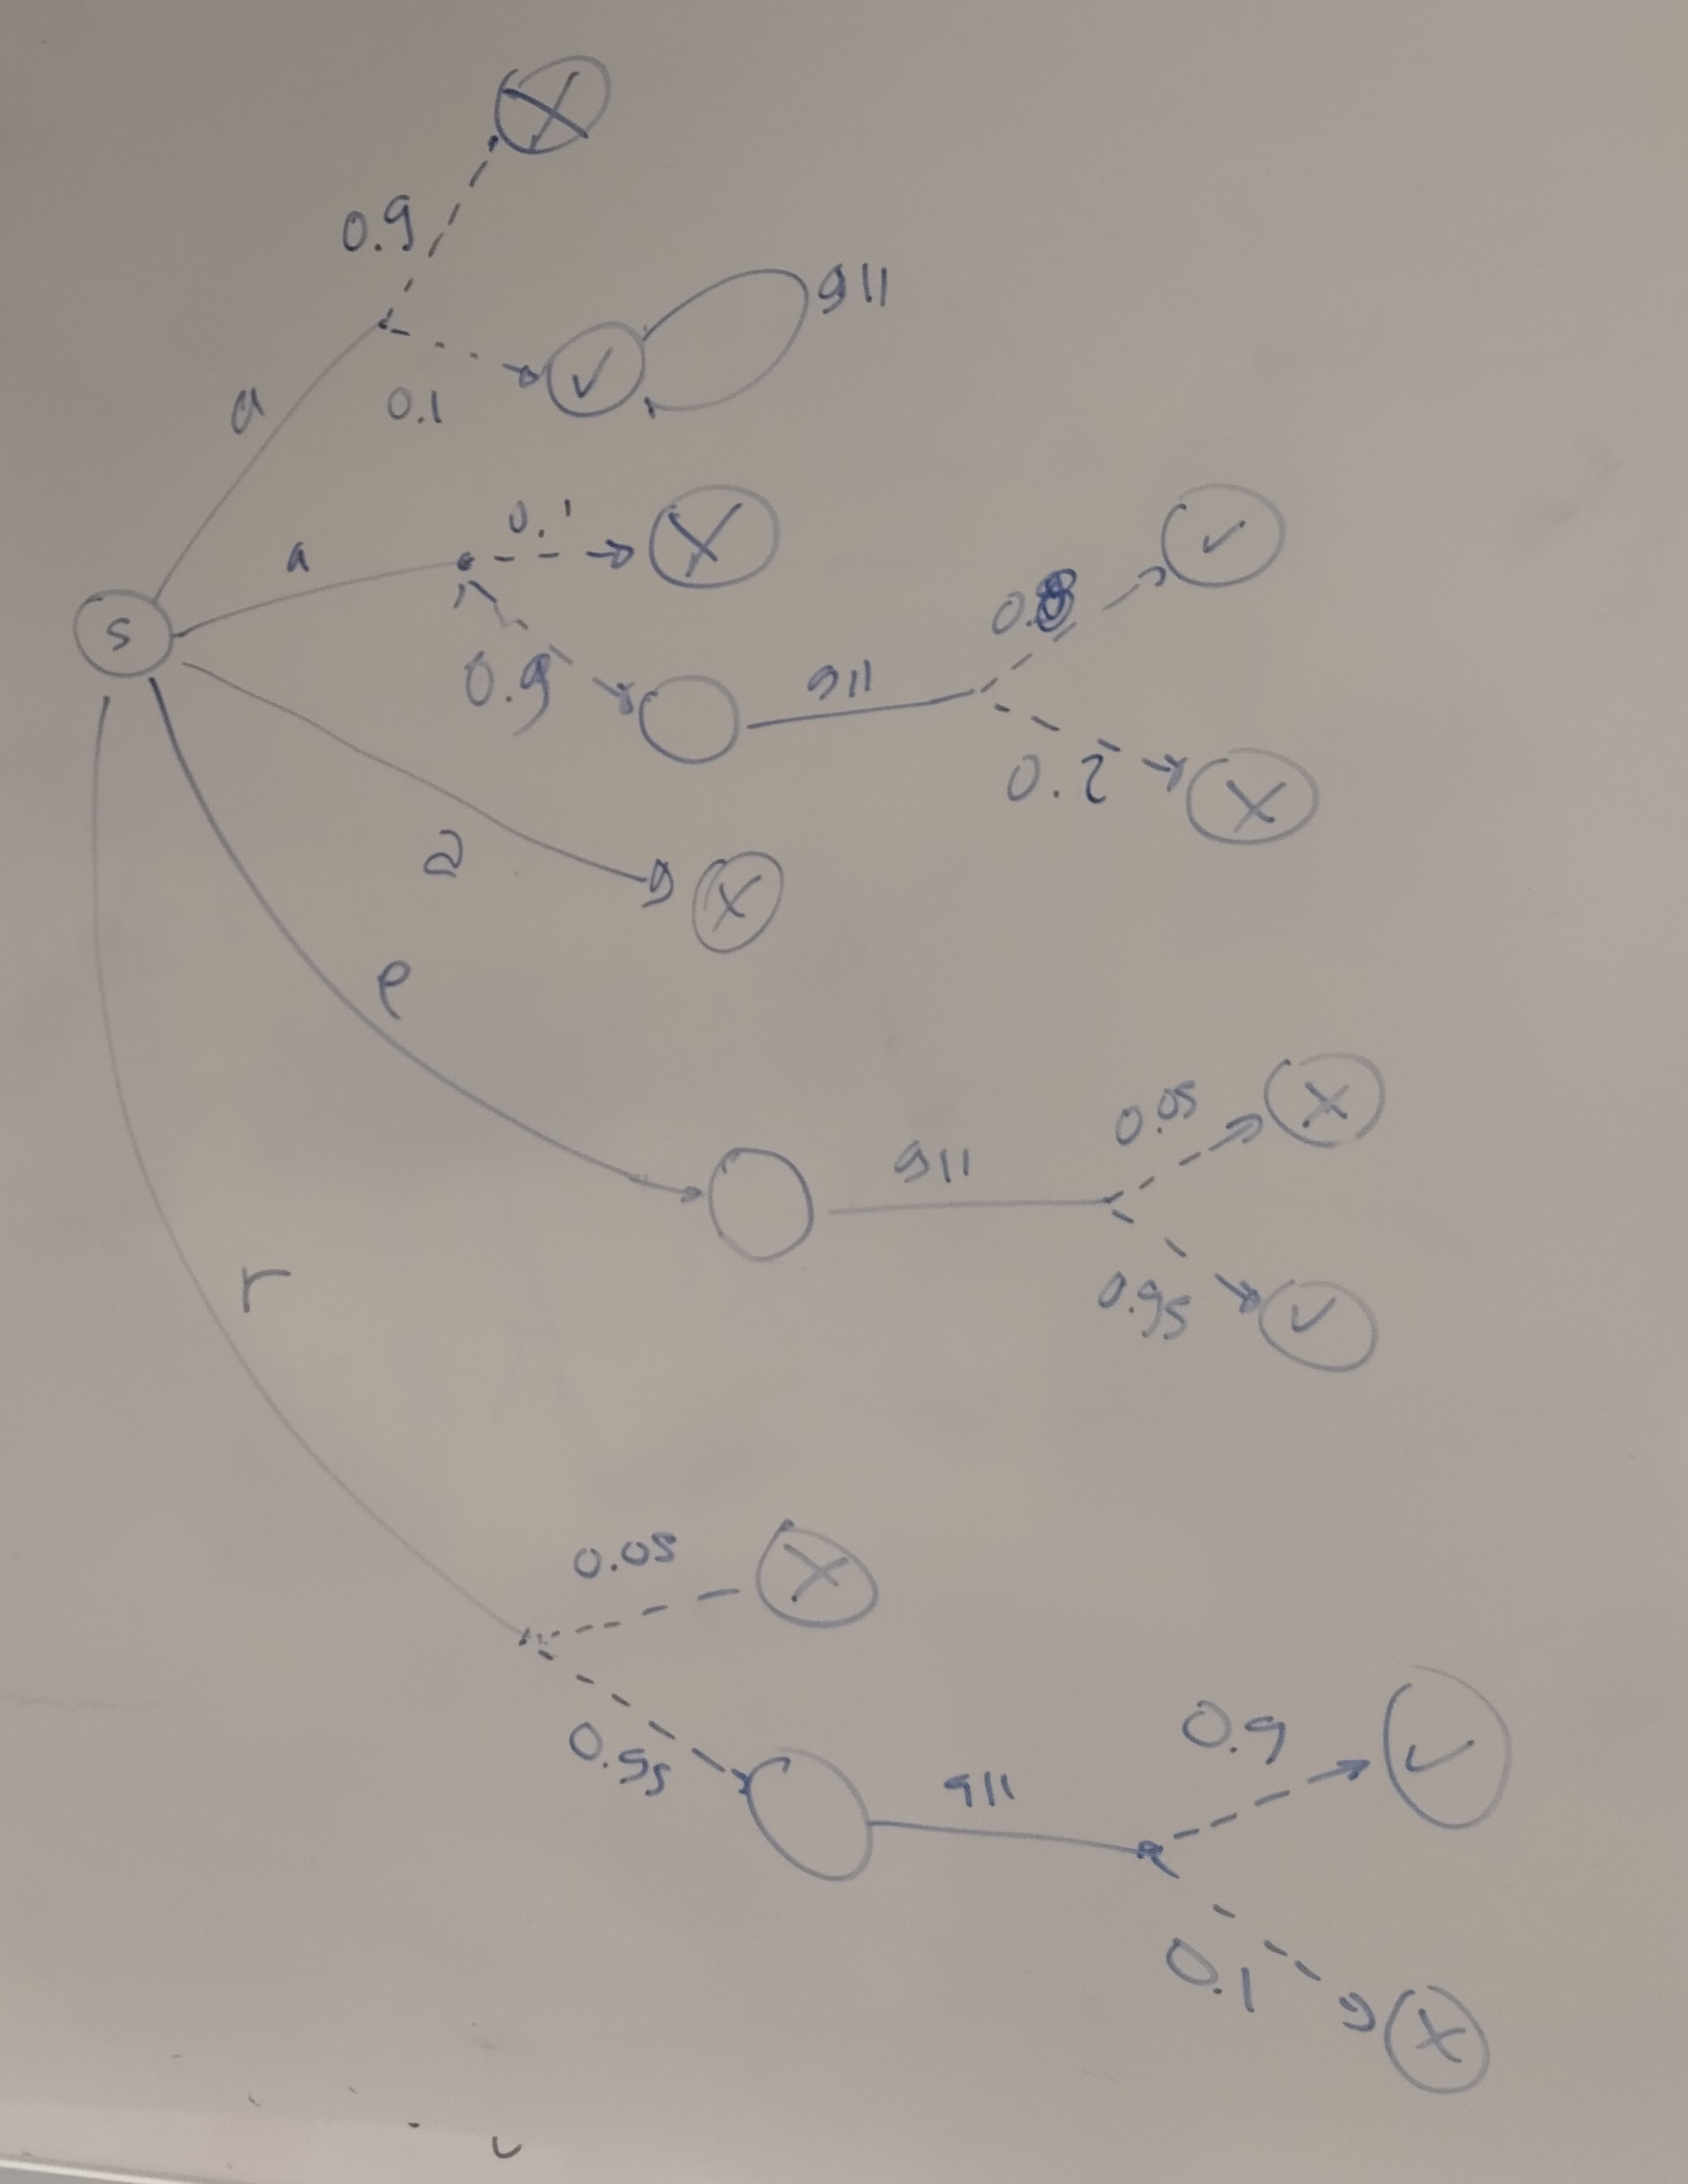
\includegraphics[scale=0.1]{PLTS.jpg}
%%     \end{center}
%% \end{figure}

% We need to capture the notion of executability with probability at least $q$, for some $q\in[0,1]$. 

% \begin{definition}\label{def:strategy-comp-exec}
%     Let $\model=\tup{\S,\Act,\ra,\V}$ be a PLTS, a \emph{strategy} is a function $\strat: \S\times(\Act\times\S)^* \ra \Dist(\S\times\Act\times\Dist(\S))$. Let $\plan\in\Act^*$, we say that $\strat$ is \emph{$\plans$-compatible} if and only if, for all $\rho\in \S\times(\Act\times\S)^*$, the following conditions hold:
%     \begin{enumerate}
%         \item $\strat(\rho)(s,a,\mu)>0$ implies $\last(\rho)=s$ and $s\reach{a}\mu$ in $\model$, and 
%         \item $\bar{\rho}\in\pref(\plans)$ implies $\bar{\rho}a\in\pref(\plans)$.
%     \end{enumerate}
%     For $\plan\in\Act^*$, we say that $\strat$ is \emph{$\plan$-compatible} if it is $\{\plan\}$-compatible. 

%     Let $q\in[0,1]$, we say that $\plans$ is \emph{$q$-executable} at $s\in\S$, if and only if, 
%     \[
%         \infim_{\{\strat \mid \strat \text{ is } \plans\text{-comp.}\}} \Prob^\strat_{s}(\plans)\geq q.
%     \]
%     Finally, $\plans$ is \emph{$q$-executable} at $B\subseteq\S$, if and only if, it is $q$-executable at every $s\in B$. 
%     A plan $\plan$ is \emph{$q$-executable} at $s$ (respectively, at $B$) if $\{\plan\}$ is $q$-executable at $s$ (respectively, at $B$). 
% \end{definition}

% \bigpedro{todo lo de arriba en esta subsecci\'on deber\'ia irse, la mayor\'ia de las cosas est\'an definidas en los preliminaries, queda la idea de $\plans$-compatible que viene debajo}



%% Given a set of plans $\plans\subseteq\Act^*$, we want to consider
%% strategies that follow as faithfully as possible the plans of
%% $\plans$.  Therefore, we say that a strategy $\strat$ is
%% \emph{$\plans$-compatible} if for all $\rho\in\execf$ such that
%% $\bar{\rho}\in\pref(\plans)$,
%% %
%% \begin{enumerate}
%% \item%
%%   $\strat(\rho)(a,\mu)>0$ implies $\bar{\rho}a\in\pref(\plans)$, and
%% \item%
%%   $\strat(\rho)(\complete)>0$ implies that either
%%   $\bar{\rho}\in\plans$ or
%%   $\bar{\rho}\{a\mid{\last(\rho)\reach{a}\mu}\}\cap\pref(\plans) = \emptyset$. 
%% \end{enumerate}
%% %
%% The first item states that $\strat$ can chose an $a$-labeled
%% transition after the partial plan $\bar{\rho}$ if the continuation of
%% $\bar{\rho}a$ is also a partial plan.
%% %
%% The second item states that $\strat$ is allowed to terminate after the
%% partial plan $\bar{\rho}$ if either $\bar{\rho}$ is itself a valid
%% plan, or $\bar{\rho}$ cannot be continued by the PLTS within some
%% valid plan.
%% %
%% Let $\Comp(\plans)$ denote the set of all $\plans$-compatible
%% strategies.
%% %
%% %% Given a plan $\plan\in\Act^*$, we say that a strategy $\strat$ is
%% %% $\plan$-compatible iff it is $\{\plan\}$-compatible.


%% Let $\plans$ be a set of plans that are believed to perform
%% equivalently in order to reach some goal state in $G\subseteq\S$.  We
%% define the set of \emph{successful complete (finite) execution} that
%% reach $G$ following some plan in $\plans$ by
%% $\Succ(\plans,G)=\{{\rho\complete\in\cexecf}\mid{\bar{\rho}\in\plans
%%   \text{ and } \last(\rho)\in G}\}$.
%% %
%% We are interested in that any $\plans$-compatible strategy $\strat$
%% starting from a given state $s\in\S$ reaches a state in $G$ with a
%% minimum desired probability, say $q$.  That is, we would like that
%% %
%% \begin{equation}\label{eq:plans:goal:q}
%%   \inf_{\strat \in\Comp(\plans)}\Prob^\strat_s(\Succ(\plans,G)) \geq q.
%% \end{equation}
%% %
%% More generally, we would like that this holds from any particularly
%% assumed state in a set $A\subseteq\S$ (say, a precondition).  So, we
%% write $A \reach{\plans}_q G$ if and only if for all state $s\in A$,
%% the condition in \cref{eq:plans:goal:q} holds.
%% %
%% Thus $A \reach{\plans}_q G$ means that any state in $A$ can reach the
%% goal $G$ with at least probability $q$ following some plan in $\plans$
%% \textcolor{red}{in an adaptively manner}.
%% \pedro{ejemplo de esto tambi\'en}


%% \bigpedro{creo que es importante pensar ahora la estructura del paper}




%% \bigpedro{desde el cartel hasta aqu\'i es nuevo}



%% Notice that, whenever $q=1$, we are in the case of SE from~\Cref{def:plans}. \raul{Chequear esto} The extended language with probabilities is given below.


%% \begin{definition}
%%     \label{def:syntax-extended}
%%     The set of formulas (a.k.a. the language) of $\Khlogic$ is defined by the following BNF:
%%     \[
%%         \varphi, \psi ::= p \mid \neg \varphi \mid \varphi \vee \psi \mid \kh^q(\psi,\varphi),
%%     \]
%%     where $p\in\Prop$ and $q\in[0,1]$. Other Boolean operators are defined as usual. Formulas of the form $\kh(\psi,\varphi)$ are read as \emph{``the agent knows how to achieve $\varphi$ given $\psi$ with probability at least $q$''}.
%% \end{definition}




%% Now we proceed by introducing the semantics of the new modality.

%% \begin{definition}
%%     \label{def:semantic-extended}
%%     Let $\model = \tup{\S,\Act,\ra,\V}$ be a PLTS and let $s\in\S$, the satisfiability relation $\models$ for $\PKh$ is inductively defined as:
%%     \[
%%         \begin{array}{l@{\ \ \ }c@{\ \ \  }l}
%%         % \model, s \models p & \iffdef & p \in \V(s) \\
%%         % \model, s\models \neg\varphi & \iffdef & \model, s \not\models \varphi \\
%%         % \model, s \models \psi\vee\varphi & \iffdef & \model, s \models \psi \mbox{ or }\model, w \models \varphi \\
%%         \model, s \models \kh^q(\psi,\varphi) & \iffdef & \text{there is } \plan \in \Act^* \;\text{such that:} \\
%%         & & \ \ \text{\rm (1)} \ \plan \text{ is $q$-executable at }  \truthset{\model}{\psi}\; \text{and} \\
%%         & & \ \ \text{\em (2)} \ \truthset{\model}{\psi} \reach{\plan}_q \truthset{\model}{\varphi}, 
%%         \end{array}
%%         \] \raul{1 and 2 will be merged into one condition.}
%%         where: $\truthset{\model}{\chi} := \csetsc{s\in\S}{\model,w\models\chi}$. Define: $\model\models\varphi$ iff  $\truthset{\model}{\varphi}=\S$, and $\models\varphi$ iff $\model\models\varphi$, for all PLTS $\model$.
%% \end{definition}

%% \begin{theorem}\label{th:mc-khp-undecidable}
%% The model-checking problem for $\PKh$ is undecidable.
%% \end{theorem}

%% \begin{proof}
%%     Suppose we want to check whether $\model,s\models\kh^q(\psi,\varphi)$.  W.l.o.g., consider $\model$ is complete and deterministic. 
%%     From the semantics, we need to check if there is $\plan\in\Act^*$ satisfying conditions (1) and (2). Consider condition (1), i.e., we need to check whether $\plan$ is $q$-executable at all $s\in\truthset{\model}{\psi}$. Fix such an $s$. Since $\model$ is deterministic and complete, it all boils down to check whether there is $\plan\in\Act^*$ such that $\Prob^\strat_s(\plan)\geq q$ (notice that $\strat$ is unique by determinism of $\model$). 
%%     The latter solves the problem of checking whether the language recognized by a probabilistic (deterministic) automata is empty, which is undecidable~\cite{MadaniHC99}. 
%% \end{proof}


%% \subsection{A First Approach: Non-Adaptive Plans}

%% The results in the above show a huge jump in the computational behaviour of knowing-how: while model-checking in the standard case is \PSPACE-complete, considering probabilities leads to undecidability of the same problem. Here, we will deal with the version of knowing-how, in which an agent only considers plans that belong to its uncertainty/awareness class. We will introduce two logics considering probabilities, one generalizing the logic from~\cite{AFSVQ21,AFSVQ23} (each plan in a class must be an appropriate plan) and another one in which it will suffice to have certain appropriate plans in a class. For the former, the model-checking problem again becomes undecidable (contrary to the \PTIME problem of the logic without probabilities, see e.g.~\cite{AFSVQ21,AFSVQ23,DF23}), while for the second, the problem is decidable. In what follows, apart from the technical results, we will motivate the use of the decidable logic in some examples.

%% Here we introduce some definitions, extending those in e.g.~\cite{AFSVQ21,AFSVQ23}.


%% \begin{definition}\label{def:plts}
%%     Let $\Prop$ be a countable set of propositional symbols and let $\AGT$ be a finite set of agents.  
%%     A \emph{Probabilistic Labeled Transition System with uncertainty (PLTSU)}  is a tuple
%%     $\model=\tup{\S,\Act,\ra,\sim,\V}$ s.t. $\tup{\S,\Act,\ra,\V}$ is a PLTS, and 
%%     \begin{itemize}
%%         % \item $\S$ is a countably non-empty set of states,
%%         % \item $\Act$ is a countable set of action symbols,
%%         % \item $\Dist(\S)$ is the set of probability distributions over $\S$,
%%         % \item ${\ra} \subseteq \S \times \Act \times \Dist(\S)$ is a transition relation,
%%         \item ${\sim}\subseteq \DS{}\times \DS{}$ (where $\DS{}\subseteq\Act^*$) is an equivalence relation over $\DS{}$. 
%%         % \item $\V: \S \ra 2^\Prop$ is a valuation function.
%%     \end{itemize}
%%     %Elements of $\Act^*$ are called \emph{plans}, and 
%%     Each $\sim$ is called the indistinguishability relation between plan. 
%%     % We write $\plan\sim_i\plan'$ whenever $(\plan,i,\plan')\in{\sim}$, and we define $\DS{i}:=\set{\plan \mid \text{ there is } \plan' \text{ s.t. } \plan\sim_i\plan'}$. 
%%     By $[\plan]_{\sim}:=\set{\plan' \in \DS{} \mid \plan \sim_i \plan'}$ we denote $\plan$'s equivalence relation with respect to $\DS{}$, then we define the \emph{indistinguishability set of $\model$} as $\Unc := \set{[\plan]_{\sim} \mid \plan\in\DS{}}$. 
%%     %The set $\Unc:=\set{\Unc(i) \mid i\in\AGT}$ is called the \emph{uncertainty set} of $\model$. 
%%     For simplicity sake, we sometimes denote $\model=\tup{\S,\Act,\ra,\Unc,\V}$ to refer to a PLTS, i.e., we will use its uncertainty set instead of the indistinguishability relation.
%% \end{definition}

%% Notice that, as it is defined in~\cite{AFSVQ21,AFSVQ23}, $\Unc$ represents the perception the agent has about the reality. In turn, the relation $\sim$ is not an equivalence relation over $\Act^*$ but over $\DS{}$, as the latter contains only the plans she considers available or suitable for her purposes, while those in $\Act^*\setminus\DS{}$ are not considered by the agent, even if they are suitable plans. 

%% % \begin{definition} \label{def:executability} \raul{TBC}
%% %     Let  $\model=\tup{\S,\Act,\Dist(\S),\ra,\Unc,\V}$ be a PLTSU, let $\plan\in\Act^*$ be a plan, and let $q\in[0,1]$ a probability, we need to define two notions:
%% %     \begin{enumerate}
%% %         \item We say $\plan$ is \emph{$q$-executable} at $s\in\S$ iff ...  Extend it for set of plans and set of states.
%% %         \item For $s,t\in\S$, we write $s \reach{\plan}_q t$ iff ... Extend it for set of plans and set of states.
%% %     \end{enumerate}
%% % \end{definition}

%% In general, we will assume that PLTS are complete, as for those we can always complete the execution of a plan to a \emph{sink state}.

%% % \begin{definition}
%% %     \label{def:syntax}
%% %     The set of formulas (a.k.a. the language) of $\PKhunc$ is defined by the following BNF:
%% %     \[
%% %         \varphi, \psi ::= p \mid \neg \varphi \mid \varphi \vee \psi \mid \kh_i^q(\psi,\varphi),
%% %     \]
%% %     where $p\in\Prop$, $i\in\AGT$ and $q\in[0,1]$. Other Boolean operators are defined as usual. Formulas of the form $\kh_i^q(\psi,\varphi)$ are read as \emph{``agent $i$ knows how to achieve $\varphi$ given $\psi$, with probability $q$''}
%% % \end{definition}

%% \begin{definition} \label{def:semantics-non-adap}
%%     Let $\model = \tup{\S,\Act,\ra,\Unc,\V}$ be a PLTSU and let $s\in\S$, the satisfiability relation $\models$ for $\PKhunc$ is inductively defined as:
%%     \[
%%     \begin{array}{l@{\ \ \ }c@{\ \ \  }l}
%%     % \model, s \models p & \iffdef & p \in \V(s) \\
%%     % \model, s\models \neg\varphi & \iffdef & \model, s \not\models \varphi \\
%%     % \model, s \models \psi\vee\varphi & \iffdef & \model, s \models \psi \mbox{ or }\model, w \models \varphi \\
%%     \model, s \models \kh^q(\psi,\varphi) & \iffdef & \text{there is } \plans \in \Unc \;\text{such that for all } \plan\in\plans{:} \\
%%     & & \ \ \text{\rm (1)} \ \plan \text{ is $q$-executable at }  \truthset{\model}{\psi}\; \text{and} \\
%%     & & \ \ \text{\em (2)} \ \truthset{\model}{\psi} \reach{\plan}_q \truthset{\model}{\varphi}, 
%%     \end{array}
%%     \]     \raul{1 and 2 to be merge into one.}
%%     \noindent where: $\truthset{\model}{\chi} := \csetsc{s\in\S}{\model,w\models\chi}$. Define: $\model\models\varphi$ iff  $\truthset{\model}{\varphi}=\S$, and $\models\varphi$ iff $\model\models\varphi$, for all PLTS $\model$.
%% \end{definition}

%% This definition bears a resemblance to the one in Section~\ref{sec:khlinearplans}, except that we ask the conditions hold for \emph{every plan} belonging to a set of indistinguishable plans $\plans$. We call this version of the logic \emph{non-adaptive} for such a reason, as the agent cannot use the ``good plans'' whenever she considers them ``equally good'' as others.  We will discuss later an alternative to this notion.

%% For this logic, we obtain a result similar to the one in the previous section.

%% \begin{theorem}\label{th:mc-khp-nadapt-undecidable}
%%     The model-checking problem for $\PKhunc$ under the semantics from Definition~\ref{def:semantics-non-adap} is undecidable.
%% \end{theorem}


%% \subsection{A Second Approach: Adaptive Plans}

%% Now we introduce a version of the logic $\PKhunc$ in which suitable plans for achieving a goal are \emph{adaptive}, in the sense that the full set $\plans$ must be $q$-executable, and not each plan $\plan\in\plans$ separately. Thus, the agent can use those plans that are good for her purposes, even in presence of non-appropriate plans that she considers indistinguishable from the good ones. \raul{Esto hay que venderlo un poco mejor.}

%% \begin{definition} \label{def:semantics-adap}
%%     Let $\model = \tup{\S,\Act,\ra,\Unc,\V}$ be a PLTSU and let $s\in\S$, the satisfiability relation $\models$ for $\PKhunc$ is inductively defined as:
%%     \[
%%     \begin{array}{l@{\ \ \ }c@{\ \ \  }l}
%%     % \model, s \models p & \iffdef & p \in \V(s) \\
%%     % \model, s\models \neg\varphi & \iffdef & \model, s \not\models \varphi \\
%%     % \model, s \models \psi\vee\varphi & \iffdef & \model, s \models \psi \mbox{ or }\model, w \models \varphi \\
%%     \model, s \models \kh^q(\psi,\varphi) & \iffdef & \text{there is } \plans \in \Unc \;\text{such that:} \\
%%     & & \ \ \text{\rm (1)} \ \plans \text{ is $q$-executable at }  \truthset{\model}{\psi}\; \text{and} \\
%%     & & \ \ \text{\em (2)} \ \truthset{\model}{\psi} \reach{\plans}_q \truthset{\model}{\varphi}, 
%%     \end{array}
%%     \]     \raul{1 and 2 to be merge into one.}
%%     \noindent where: $\truthset{\model}{\chi} := \csetsc{s\in\S}{\model,w\models\chi}$. Define: $\model\models\varphi$ iff  $\truthset{\model}{\varphi}=\S$, and $\models\varphi$ iff $\model\models\varphi$, for all PLTS $\model$.
%% \end{definition}

%% The general idea in condition 1 of the clause for $\kh$ establishes that all the plans in $\plans$ have a probablity of at least $q$ of succeeding. Since all plans in $\plans$ are indistinguishability, this needs to be guaranteed no matter which plan is chosen. However, there are at least two alternatives in this definition: one considering \emph{adaptability}, meaning that there is at least one possible execution of each plan in $\plans$ for which probability $q$ is guaranteed, and considering \emph{non-adaptability} whenever we need this guarantee on each possible execution of every plan in $\plans$. Condition 2 establishes that successfull states are reached with probability of at least $q$.

%% \begin{remark}
%%     Notice that an equivalence class $\plans$ can be defined in terms of a Deterministic Finite State Automata (DFA) $\mathcal{A}_{\plans}$. This way, the operation of checking $q$-executability can be perfomed over the product $\model\times\mathcal{A}_{\plans}$. In short, $\plans$ is $q$-executable at $s$ iff for each $\plan\in\plans$, there exists one MDP in  $\model\times\mathcal{A}_{\plans}$ in which the probability of executing $\plan$ is at least $q$. This will be used while designing a model-checking algorithm (connected with algorithms from~\cite{AFSVQ21,AFSVQ23,DF23}).
%% \end{remark}

%% \begin{theorem}\label{th:mc-khp-adapt-decidable}
%%     The model-checking problem for $\PKhunc$ under the semantics from Definition~\ref{def:semantics-adap} is decidable. Moreover, if each $\plans\in\Unc$ is given as input as a deterministic FSA, the problem is in $\PTIME$.
%% \end{theorem}
